
%% bare_jrnl.tex
%% V1.4b
%% 2015/08/26
%% by Michael Shell
%% see http://www.michaelshell.org/
%% for current contact information.
%%
%% This is a skeleton file demonstrating the use of IEEEtran.cls
%% (requires IEEEtran.cls version 1.8b or later) with an IEEE
%% journal paper.
%%
%% Support sites:
%% http://www.michaelshell.org/tex/ieeetran/
%% http://www.ctan.org/pkg/ieeetran
%% and
%% http://www.ieee.org/

%%*************************************************************************
%% Legal Notice:
%% This code is offered as-is without any warranty either expressed or
%% implied; without even the implied warranty of MERCHANTABILITY or
%% FITNESS FOR A PARTICULAR PURPOSE! 
%% User assumes all risk.
%% In no event shall the IEEE or any contributor to this code be liable for
%% any damages or losses, including, but not limited to, incidental,
%% consequential, or any other damages, resulting from the use or misuse
%% of any information contained here.
%%
%% All comments are the opinions of their respective authors and are not
%% necessarily endorsed by the IEEE.
%%
%% This work is distributed under the LaTeX Project Public License (LPPL)
%% ( http://www.latex-project.org/ ) version 1.3, and may be freely used,
%% distributed and modified. A copy of the LPPL, version 1.3, is included
%% in the base LaTeX documentation of all distributions of LaTeX released
%% 2003/12/01 or later.
%% Retain all contribution notices and credits.
%% ** Modified files should be clearly indicated as such, including  **
%% ** renaming them and changing author support contact information. **
%%*************************************************************************

\documentclass[journal]{IEEEtran}

% *** OWN PACKAGES ***

%\usepackage[american,siunitx, RPvoltages]{circuitikz}
\usepackage{layouts}
\usepackage{placeins}
\usepackage{textgreek}
\usepackage{tabularx}

\usepackage[american,siunitx]{circuitikz}
%\usepackage[style=IEEE,sorting=ydnt,defernumbers,backend=biber]{biblatex}

%%%%%%%%%%%%%%%%%%%
%Pakete Mathematik
\usepackage{mathtools} % erweiterte Fassung von amsmath
\usepackage{amssymb}   % erweiterter Zeichensatz
\usepackage{bm}			% fette Mathe symbole
\usepackage{siunitx}   % Einheiten
\DeclareSIUnit{\nothing}{\relax}
\sisetup{number-unit-product = \text{}}

%%%%%%%%%%%%%%%%%%%
%Pakete Pseudocode
\usepackage{algorithm}
\usepackage[noend]{algpseudocode}

% *** CITATION PACKAGES ***
%
\usepackage{cite}

% *** GRAPHICS RELATED PACKAGES ***
%
\ifCLASSINFOpdf
  % \usepackage[pdftex]{graphicx}
  % declare the path(s) where your graphic files are
  % \graphicspath{{../pdf/}{../jpeg/}}
  % and their extensions so you won't have to specify these with
  % every instance of \includegraphics
  % \DeclareGraphicsExtensions{.pdf,.jpeg,.png}
\else
  % or other class option (dvipsone, dvipdf, if not using dvips). graphicx
  % will default to the driver specified in the system graphics.cfg if no
  % driver is specified.
  % \usepackage[dvips]{graphicx}
  % declare the path(s) where your graphic files are
  % \graphicspath{{../eps/}}
  % and their extensions so you won't have to specify these with
  % every instance of \includegraphics
  % \DeclareGraphicsExtensions{.eps}
\fi

\usepackage{amsmath}

% *** SUBFIGURE PACKAGES ***
\ifCLASSOPTIONcompsoc
  \usepackage[caption=false,font=normalsize,labelfont=sf,textfont=sf]{subfig}
\else
  \usepackage[caption=false,font=footnotesize]{subfig}
\fi

% correct bad hyphenation here
\hyphenation{op-tical net-works semi-conduc-tor}
\graphicspath{ {./images/} }


\begin{document}
%

% Do not put math or special symbols in the title.
\title{FELIS-MOR Documentation}
%
%

%

\author{Frederik~Quetscher}% <-this % stops a space
% <-this % stops a space
% <-this % stops a space


% The paper headers
\markboth{IEEE template,~Vol.~$n$, No.~$m$, August~2022}%
{Shell \MakeLowercase{\textit{et al.}}: Bare Demo of IEEEtran.cls for IEEE Journals}
% The only time the second header will appear is for the odd numbered pages
% after the title page when using the twoside option.
% 
% *** Note that you probably will NOT want to include the author's ***
% *** name in the headers of peer review papers.                   ***
% You can use \ifCLASSOPTIONpeerreview for conditional compilation here if
% you desire.

\newcommand{\diff}[1][V]{\ensuremath{\,\mathrm{d}{#1}}}
\newcommand{\tensor}[1]{\ensuremath{\mathbf{#1}}}
\newcommand{\transpose}[1]{\ensuremath{{#1}^\mathsf{T}}}
\newcommand{\hermite}[1]{\ensuremath{{#1}^\mathsf{H}}}
\newcommand{\curl}{\,\mathrm{curl}\,}
\renewcommand{\div}{\,\mathrm{div}\,}
\newcommand{\grad}{\,\mathrm{grad}\,}

% make the title area
\maketitle


%%%%%%%Commands
%general
\newcommand{\mbf}{\mathbf}
\newcommand{\mrm}{\mathrm}
%\newcommand{\ul}{\underline}



%elementary sets
\newcommand{\R}{\mathbb R}
\newcommand{\Cset}{\mathbb C}
%\newcommand{\N}{\mathbb N}

%advanced sets
\newcommand{\Pcal}{\mathcal P}

\newcommand{\Dc}{\mathcal D}

\newcommand{\setFRange}{d_f}

\newcommand{\setFRF}{\mathcal F} %A^\mathrm{FRF}
\newcommand{\setFRFApp}{\mathcal F^\mathrm{Appr}} %A^\mathrm{FRF}
\newcommand{\setFRFMapped}{\Fhat{\mathcal F}} %A^\mathrm{FRF}
\newcommand{\setFRFAppMapped}{\Fhat{\mathcal F^\mathrm{Appr}}} %A^\mathrm{FRF}

\newcommand{\setSim}{\mathcal A}%^\mathrm{Sim}
\newcommand{\setApp}{\mathcal A^\mathrm{Appr}}
\newcommand{\setAppC}{\ul{\mathcal A}^\mathrm{Appr}}

\newcommand{\setFRFD}{\mathbf F} %A^\mathrm{FRF}
\newcommand{\setFRFAppD}{\mathbf F^\mathrm{Appr}} %A^\mathrm{FRF}

\newcommand{\setSimD}{\mathbf A} %^\mathrm{Sim}
\newcommand{\setAppD}{\mathbf A^\mathrm{Appr}}

\newcommand{\setCoeffApp}{\mathcal C^\mathrm{Appr}}%^\mathrm{Sim}

%operators
\newcommand{\E}{\mathrm E}
\newcommand{\re}{\mathrm{real}}
\newcommand{\im}{\mathrm{imag}}
\newcommand{\argmax}[1]{\underset{#1}{\arg\max}}
\newcommand{\argmin}[1]{\underset{#1}{\arg\min}}


%functions
\newcommand{\deltaij}{\delta_{ij}}

%variables
\newcommand{\bfx}{\mathbf x}
\newcommand{\bfy}{\mathbf y}
\newcommand{\bfY}{\mathbf Y}
\newcommand{\bff}{\mathbf f}
\newcommand{\bfh}{\mathbf h}
\newcommand{\bfH}{\mathbf H}

%words/misc

\newcommand{\gdm}{\mathrm{GDM}}
\newcommand{\with}{\ \mathrm{with}\ }
%\newcommand*{\Fhat}[1]{#1\kern-0.68em\hat{\phantom{#1}}}
\newcommand*{\Fhat}[1]{\hat{#1}}

%\newcommand*{\fhat}[1]{#1\kern-0.5em\hat{\phantom{#1}}}
%\newcommand*{\todo}[1]{\textcolor{red}{(todo: #1)}}
\newcommand*{\todo}[1]{}


\newcommand{\refgl}[1]{(\ref{#1})}
\newcommand{\mhz}[1]{\qty{#1}{MHz}}
\newcommand{\khz}[1]{\qty{#1}{kHz}}
\newcommand{\mum}[1]{#1µm}

\newcommand{\e}{\mrm e}


\newcommand{\ltn}{$L^2$-norm }


% As a general rule, do not put math, special symbols or citations
% in the abstract or keywords.
%\begin{abstract}
%\input{abstract.tex}
%\end{abstract}

% Note that keywords are not normally used for peerreview papers.
%\begin{IEEEkeywords}
%IEEE, IEEEtran, journal, \LaTeX, paper, template.
%\end{IEEEkeywords}


\IEEEpeerreviewmaketitle


















\section{MOR Stage 2}

\subsubsection{Affine decomposition for volumetric matrices+ports}
The code is available in the commit 'MOR Stage 2+documentation' of 5.12.22. The code exploits the affine decomposition 
\begin{equation}
	A_{closed}=CC+\theta_1(f)M_E+\theta_2(f)M_C,
\end{equation}
for the closed problem and the decomposition
\begin{equation}
	P_{i,red}=U^\top P_i U = U^\top p_i p_i^\top U = (U^\top p_i) (U^\top p_i)^\top
\end{equation}
for the ports. This reduces the number of operations from two matrix-matrix products to just two matrix-vector products and one outer vector-vector product with low dimensions\\

 The reduced system matrix $A_{red}$ is assembled as $A_{red}=A_{closed,red}+P_{red}$..\\
 
\subsubsection{Affine decomposition for SibcE}
Currently the computation of the SibcE is computed for each frequency point as follows:
\begin{algorithmic}[1]
	\State Select a surface element
	\State Calculate impedance on this surface (material s piecewise constant)
	\State Calculate local matrix (by using the calculated impedance)
	\State Transform local matrix to a global one
	\State Add global element matrix to the global Sibc-Matrix
\end{algorithmic}
Instead I propose to create and store for each surface a global matrix for each surface. Then for each frequency, the surface matrices have to be multiplied with their corresponding impedance and added together. To me this seems more efficient and since the Sibc matrix is much sparser than the system-matrix, it should not be problematic for the memory. If only one resistive material and pec is used, then this decomposition consists of only one matrix and impedance. So it can be used for model problems without modifications.
\\

\subsubsection{other infos}
The right hand side is taken directly from FELIS, this has to be improved in stage 3. The computation of the residual also exploits the shown decomposition of the port matrices.

The snapshots are placed equidistantly.

\subsection{results}
\subsubsection{Square Cavity}
The convergence is monitored for the residual, but also for the absolute error in the solution against a test set consisting of 250 equidistantly spaced solutions. The evaluation points are spaced according to a 1D latin hypercube (latin line?) to not be equal the training data for $m=50$.


\begin{figure}[h]
	\centering
	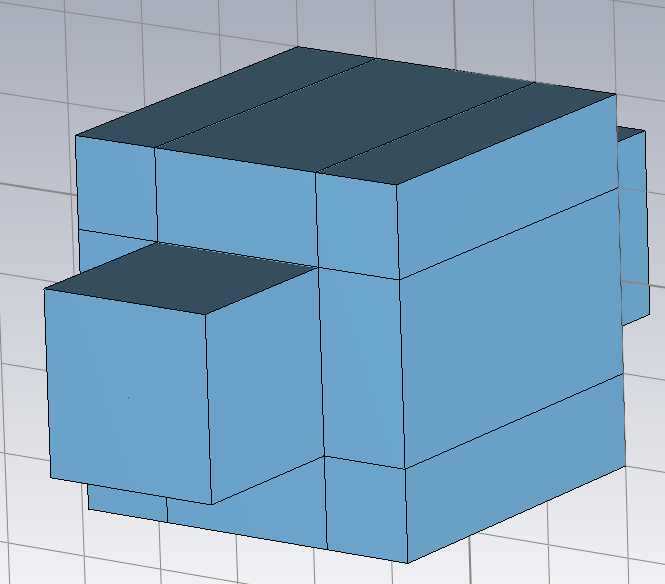
\includegraphics[width=0.5\textwidth]{SquareCavityGeo.PNG}
	\caption{Geometry of the square cavity.}
	\label{}
\end{figure}

\begin{figure}[h]
	\centering
	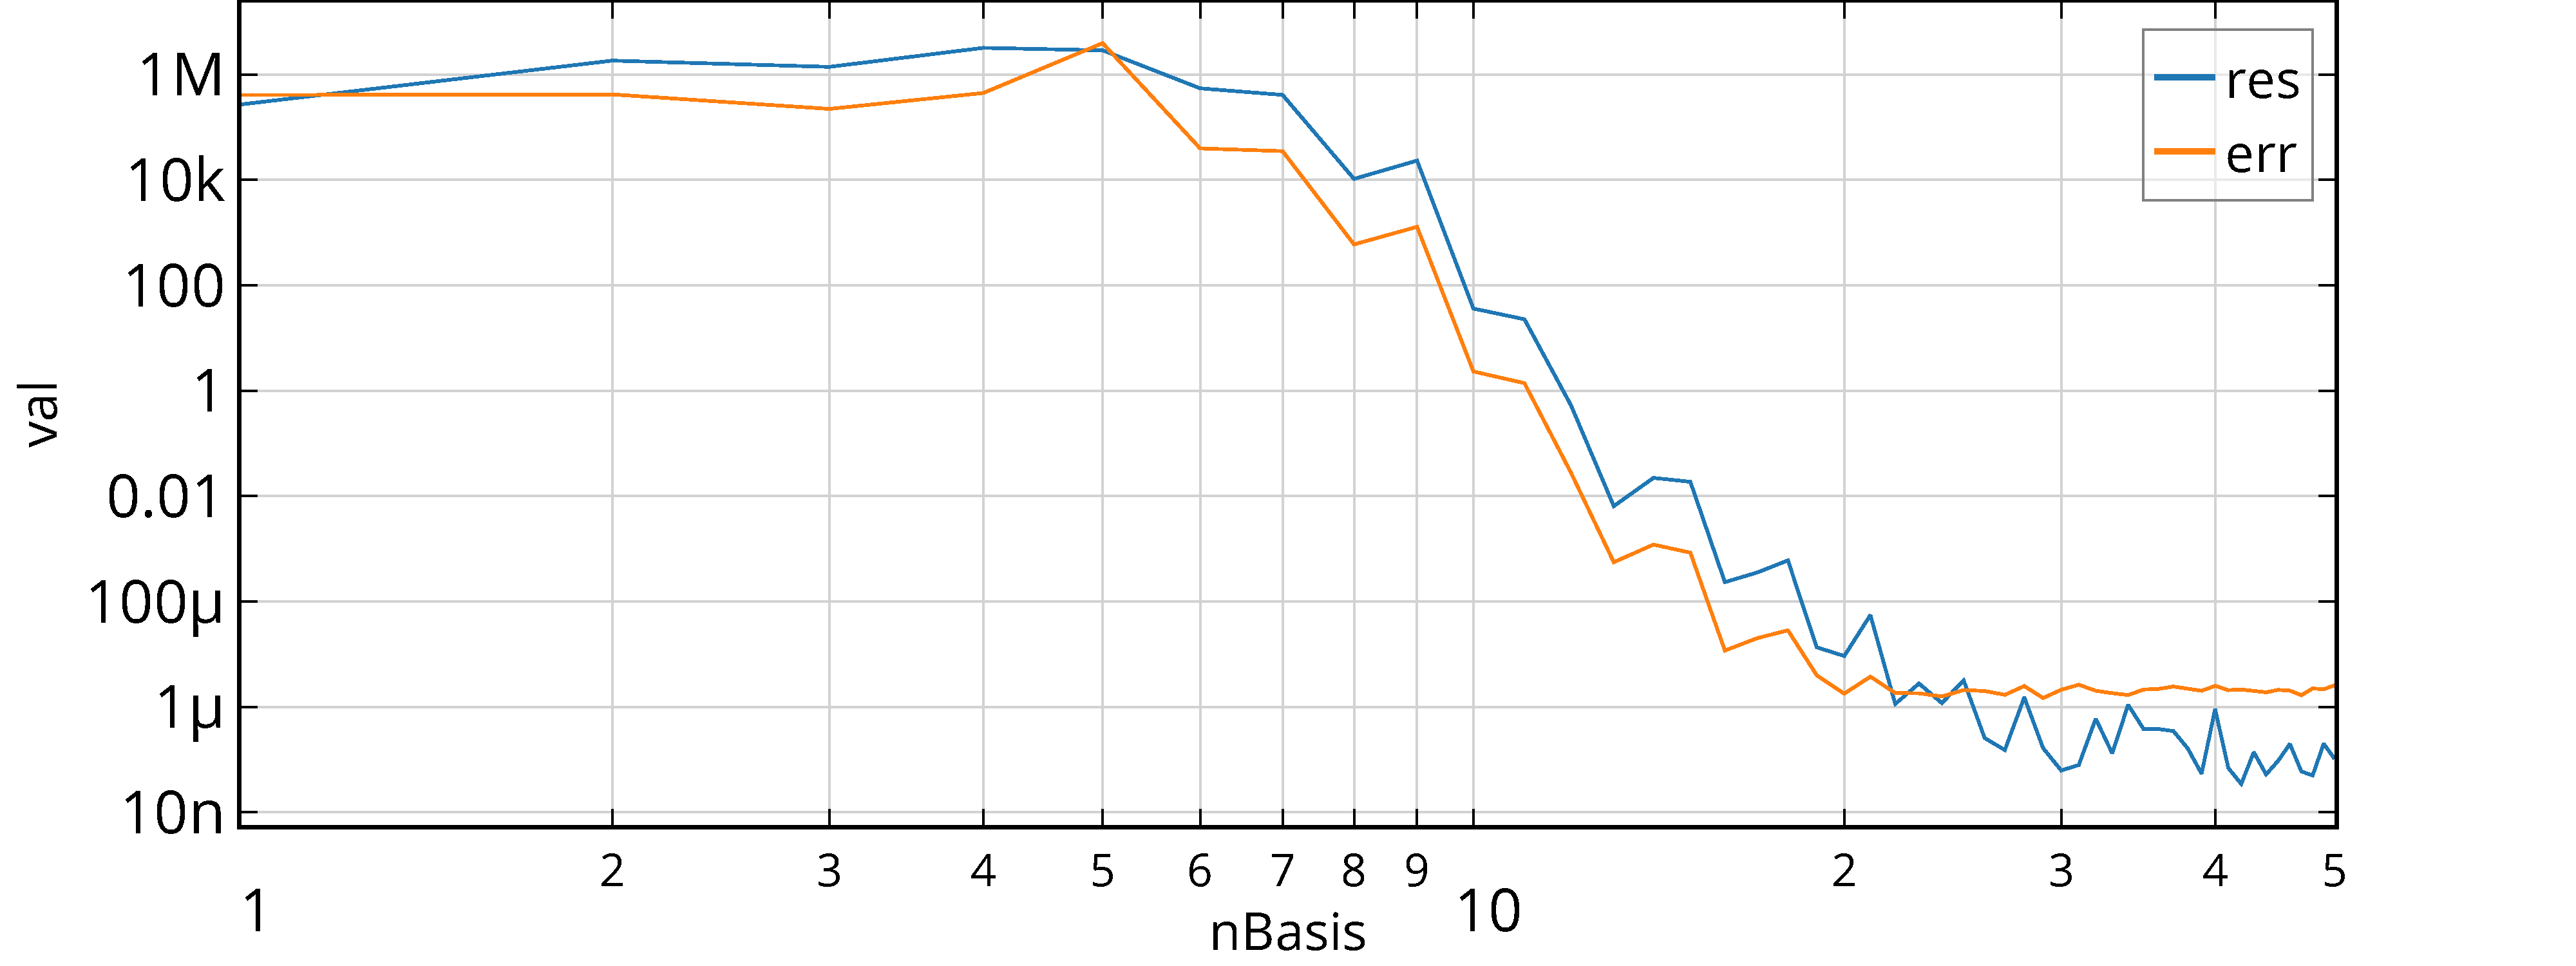
\includegraphics[width=0.5\textwidth]{sqc_conv_st2_1.pdf}
	\caption{The required number of snapshots is in the range of 5 to 20 for this example. There is a perfect agreement between the RHS residual and the error against the test-data. Hence both error metrics are viable.}
	\label{}
\end{figure}
\begin{figure}[h]
	\centering
	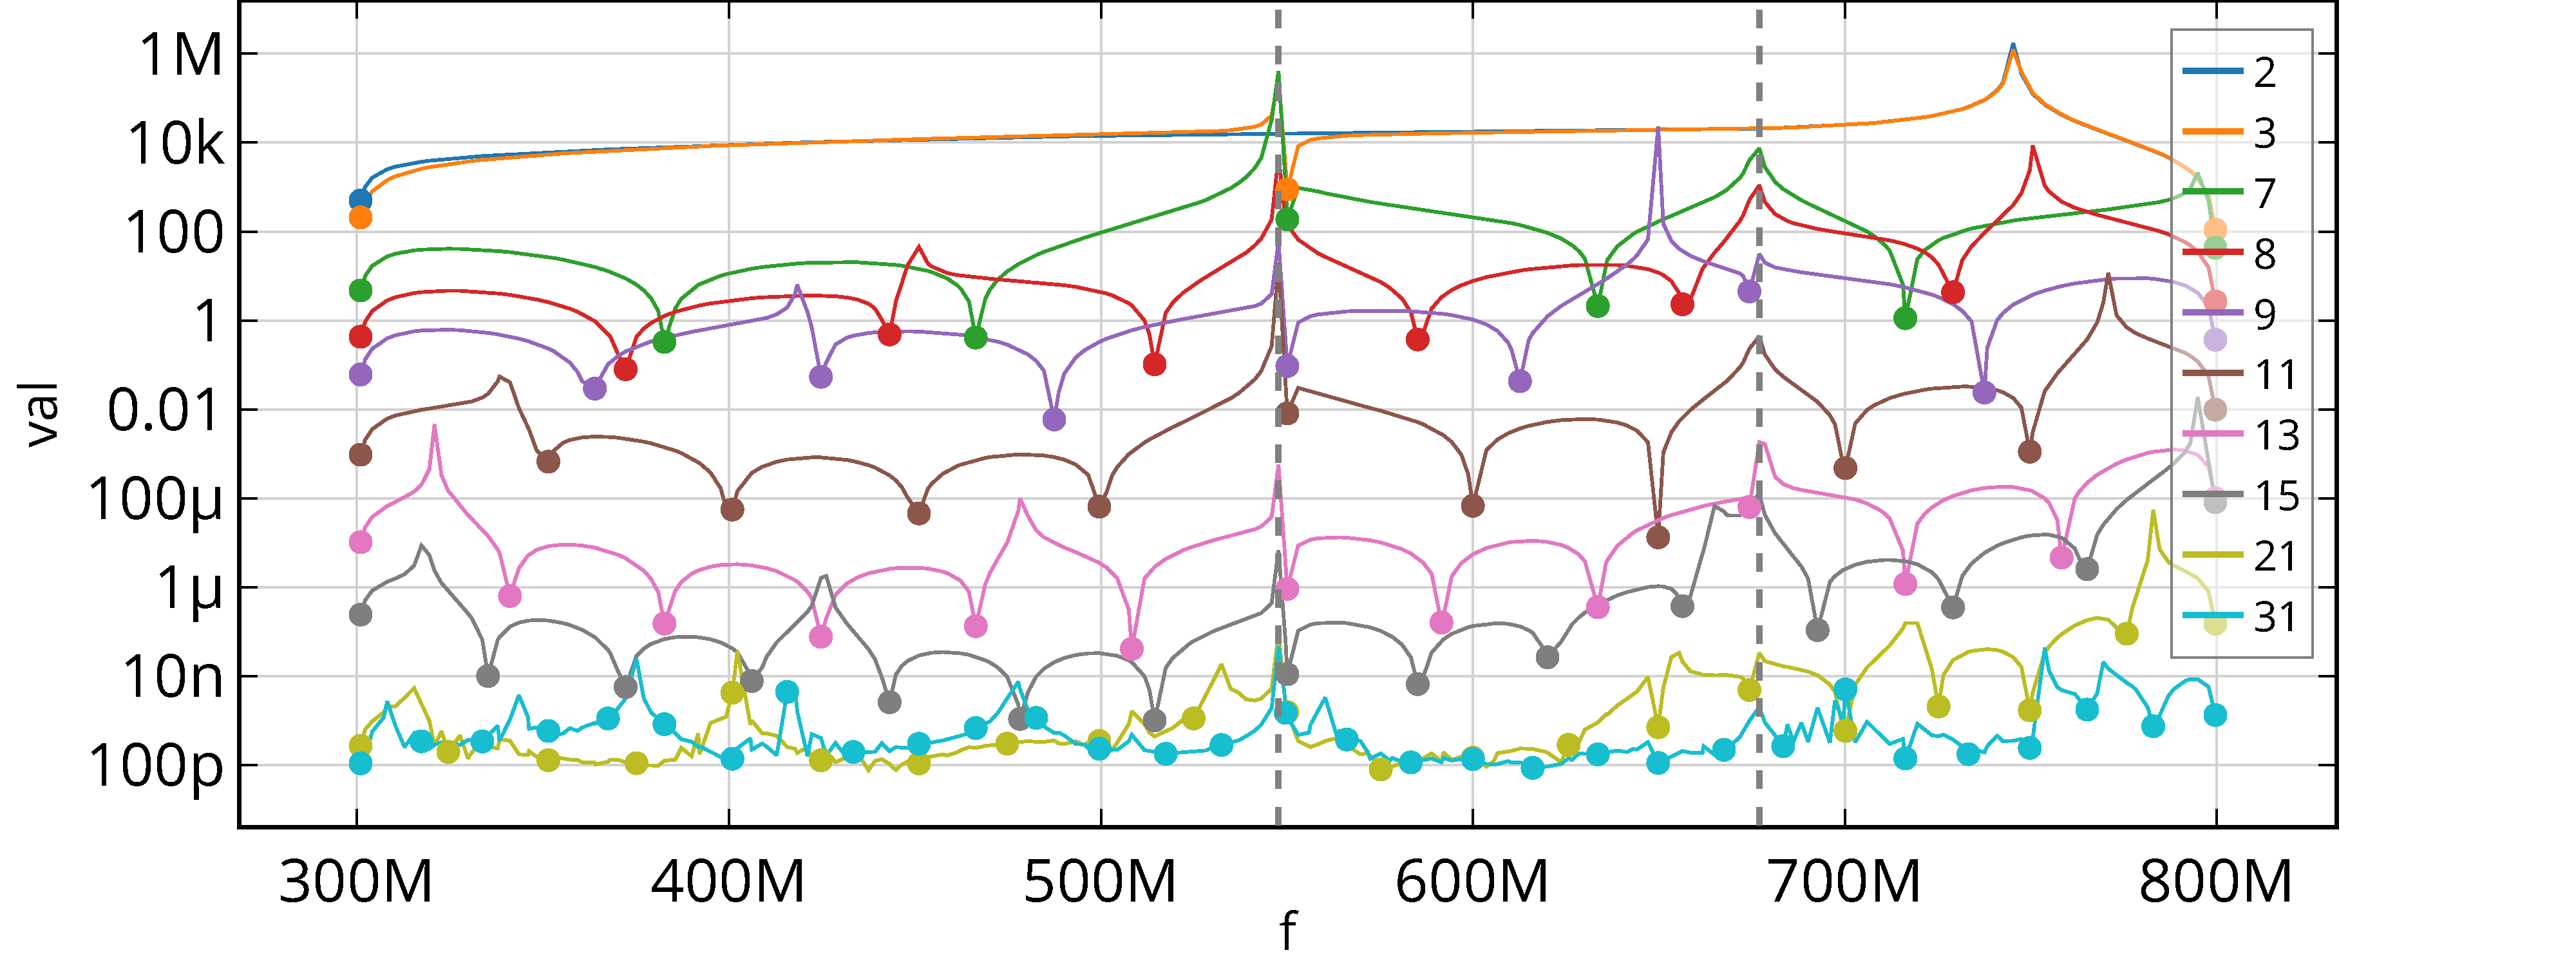
\includegraphics[width=0.5\textwidth]{sqc_conv_st2_2.pdf}
	\caption{The residual is almost frequency independent, hence an adaptive sweep would not improve convergence. The use of nested points would be more advantageous. An exception to this is the accuracy close to the resonances before convergence starts, there adaptive points may be beneficial.}
	\label{}
\end{figure}
\begin{figure}[h]
	\centering
	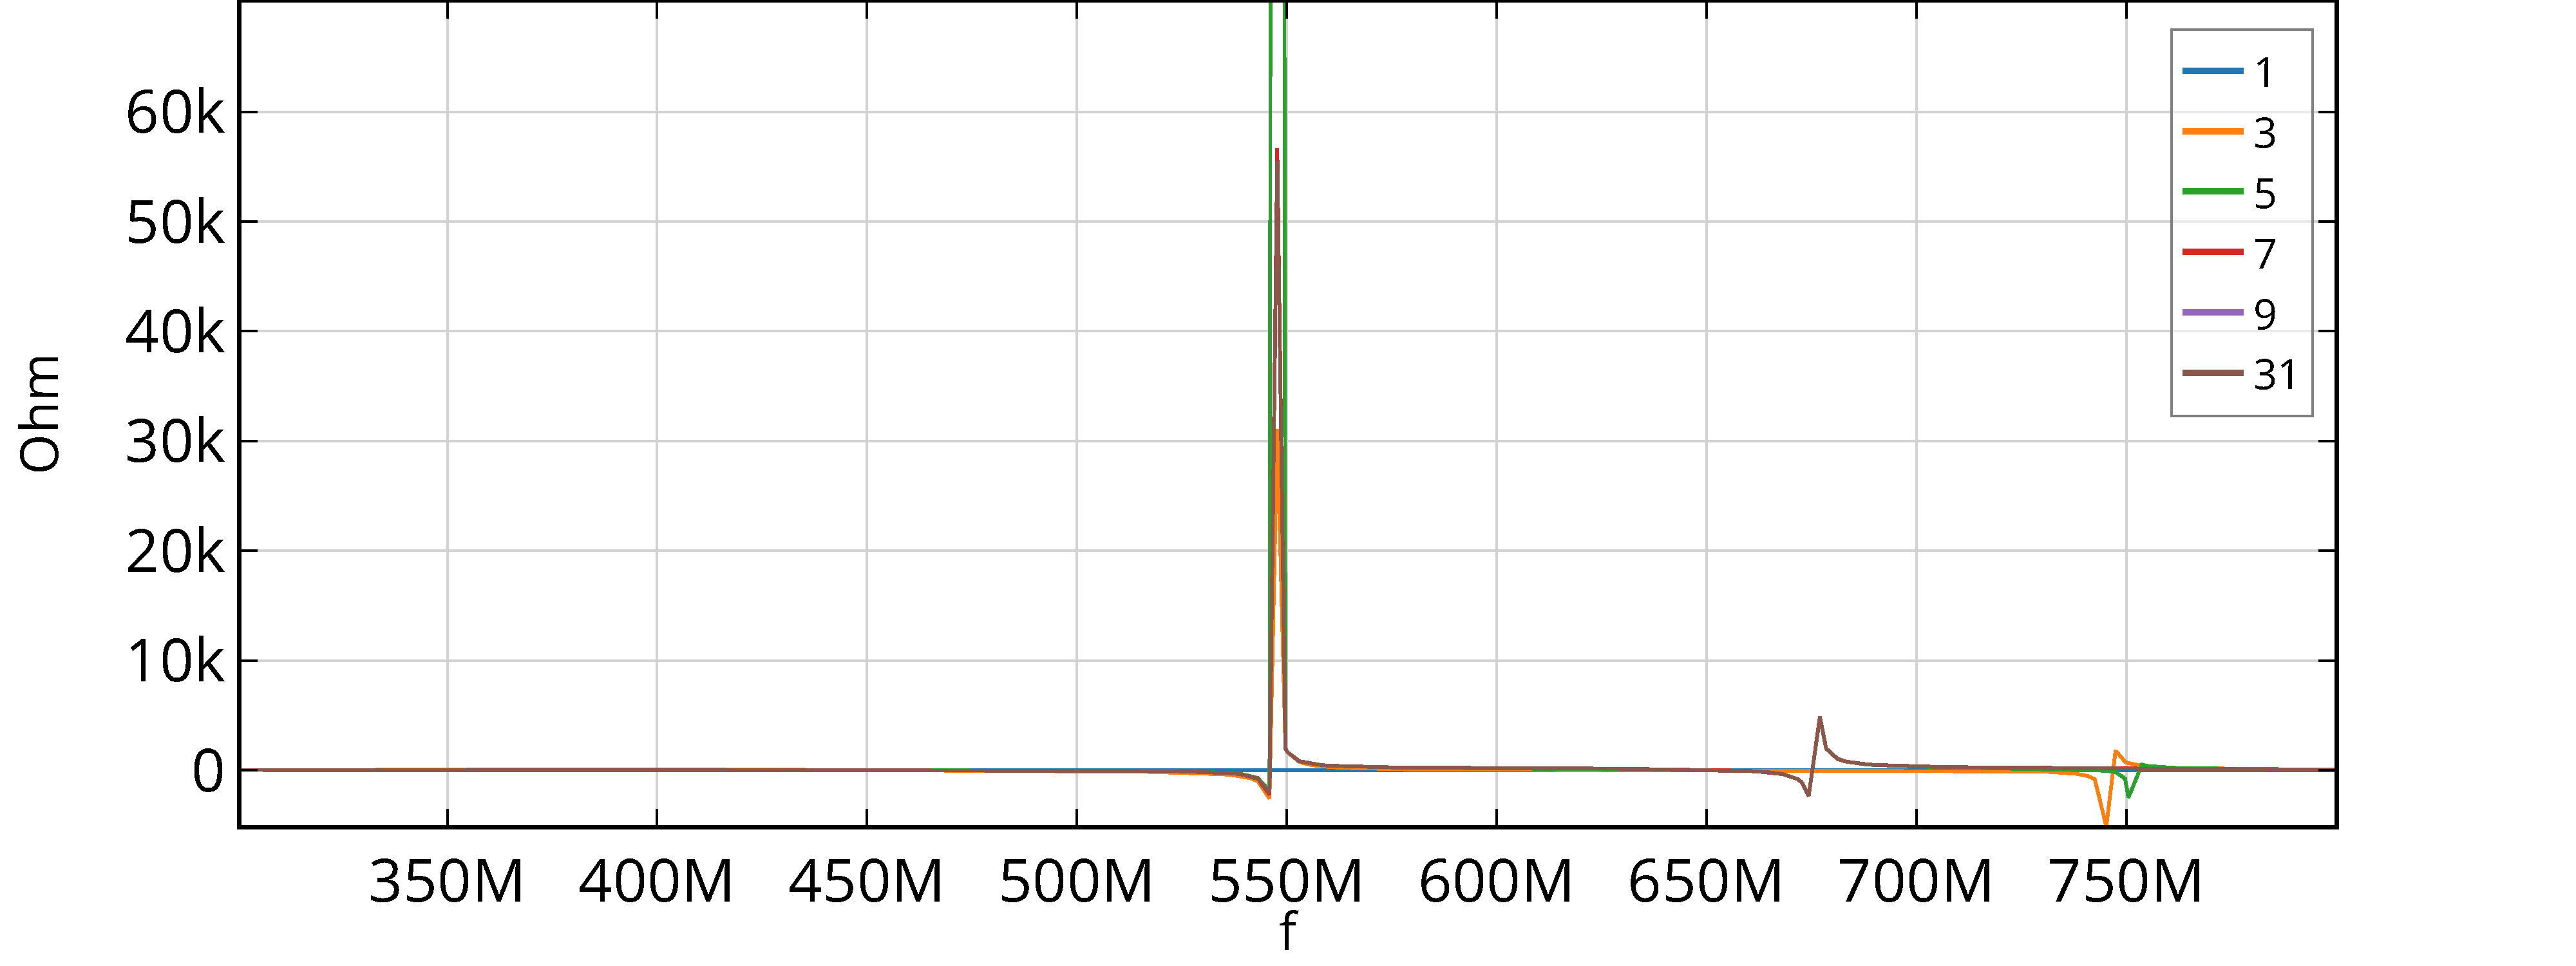
\includegraphics[width=0.5\textwidth]{sqc_imp_MOR_IM.pdf}
	\caption{Imaginary part of the impedance. The first resonance frequency is met to full visual accuracy at nB=3, the second at nB= 7. At nB=7 no further convergence is visible.}
	\label{}
\end{figure}

\begin{figure}[h]
	\centering
	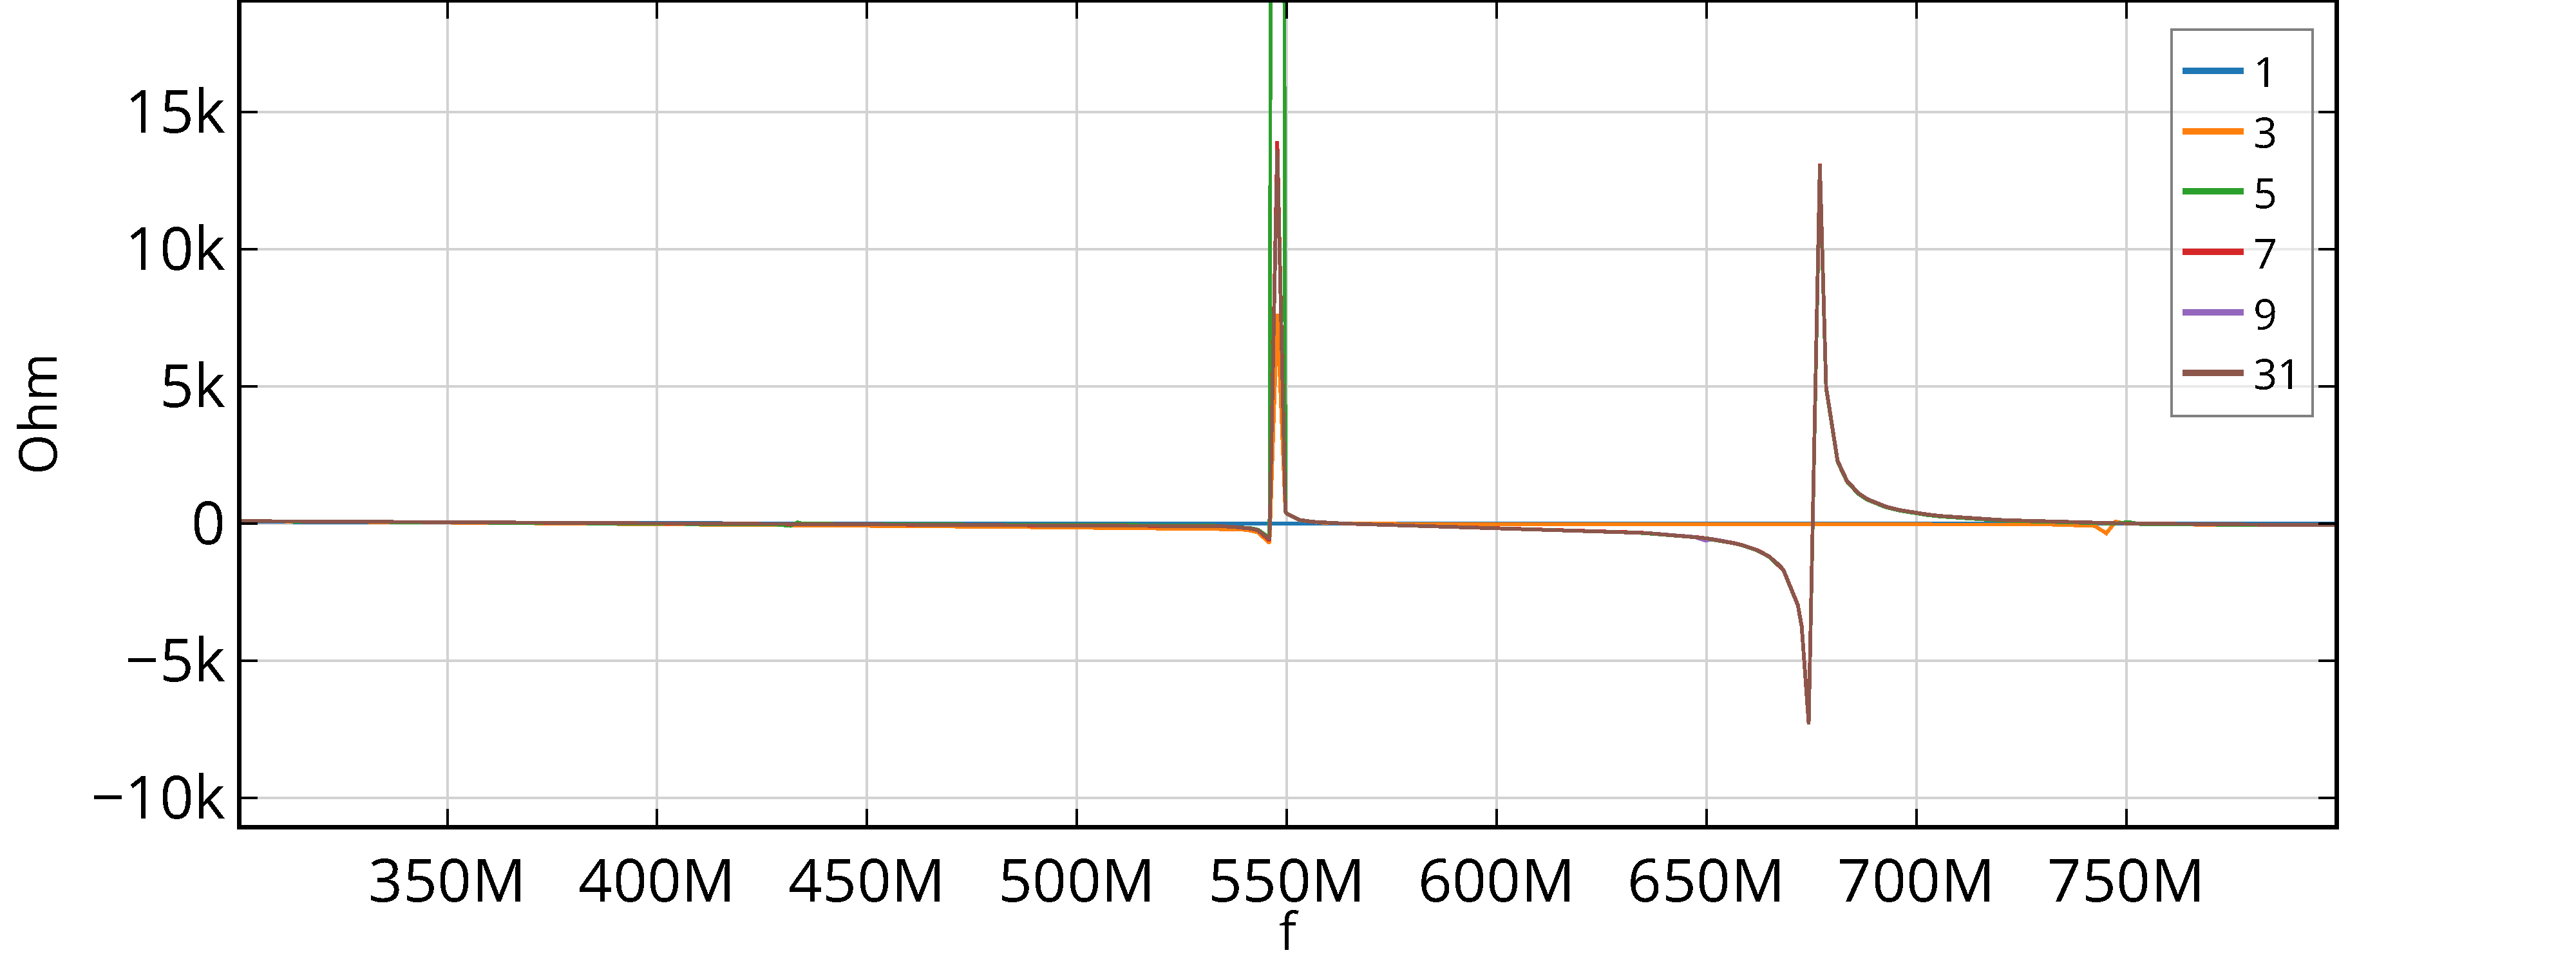
\includegraphics[width=0.5\textwidth]{sqc_imp_MOR_RE.pdf}
	\caption{Real part of the impedance. About the same observations regarding the convergence. Main observation: The real part does not agree with the FELIS code (Zre=0), but agrees with CST (if I remember correctly). Also if I calculate the impedance in Matlab using the field solution and current density exported from FELIS, I get this result. Is there maybe a mistake in FELIS? Update: Im python code war noch ein Fehler, jetzt könnten Felis und python übereinstimmen}
	\label{}
\end{figure}

\begin{figure}[h]
	\centering
	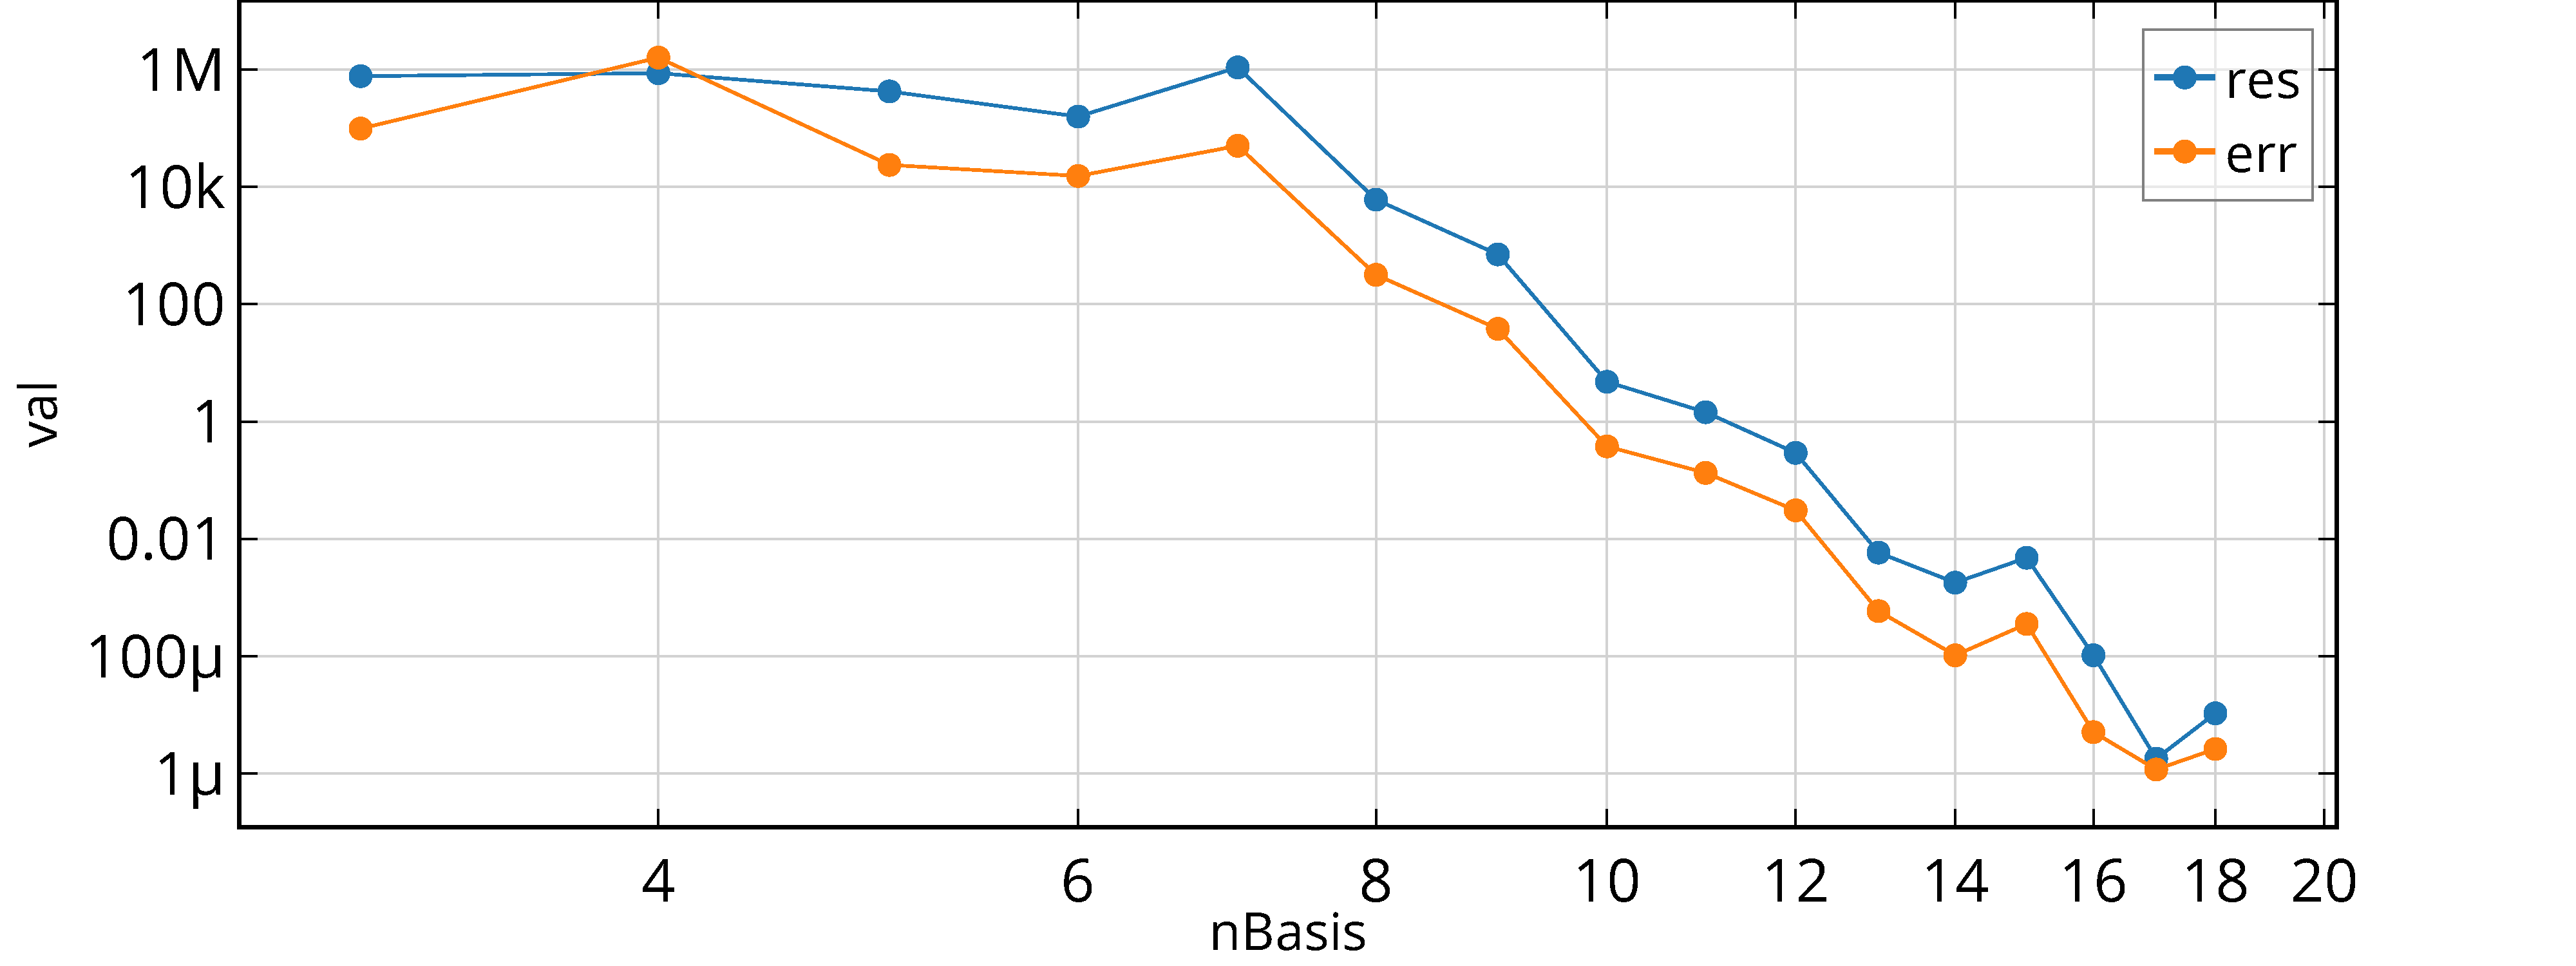
\includegraphics[width=0.5\textwidth]{sqc_conv_st2_adap_1.pdf}
	\caption{Convergence if always the frequency with largest residual gets added. The convergence is slightly faster. Compare to linearly spaced problem, looking at err: For nB=8 both samplings lead to the same error. The adaptive sampling reaches at nB=16 the full accuracy, the linear one at nB=19. The adaptive sampling breaks down, because a previously chosen frequency point is chosen again.}
	\label{}
\end{figure}


\begin{figure}[h]
	\centering
	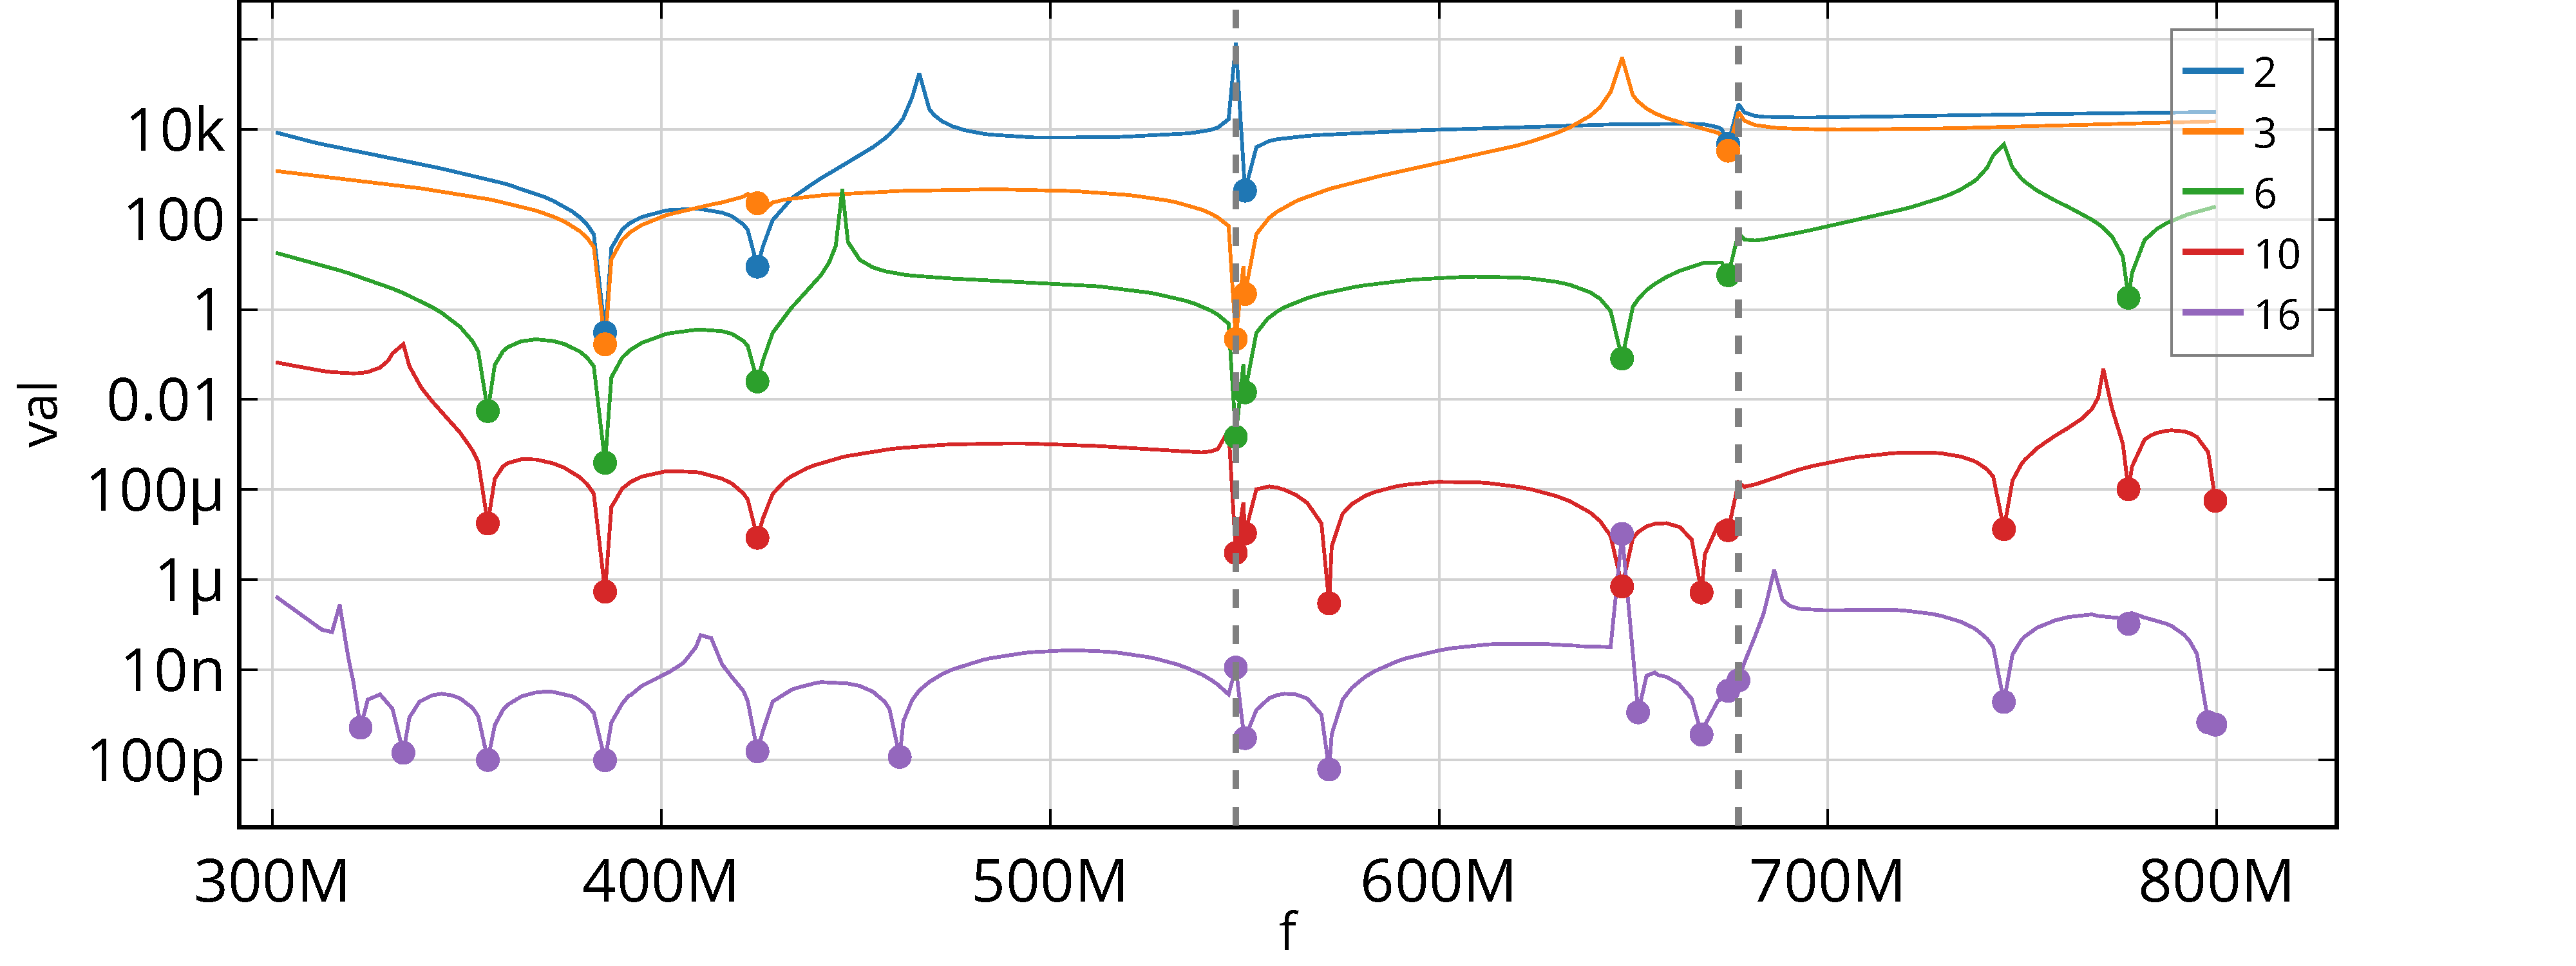
\includegraphics[width=0.5\textwidth]{sqc_conv_st2_adap_2.pdf}
	\caption{Convergence of the residual over the frequency axis. The dots show the frequencies where the snapshots are taken. The algorithm breaks down, because the sample at around 660MHz is chosen again.\\
	As visible: 1. the convergence is not uniform; 2. the spacing is surprisingly close to uniform; 3. almost always the residual is the lowest at the snapshots. Interestingly the technique of sampling at the highest residual is similar to an adaptive Gram-Schmidt method. A faster and more uniform convergence may be achieved, if the samples would be taken at the frequencies of highest expected improvement. This is actually the idea behind the SVD.}
	\label{}
\end{figure}
 
 
 \begin{figure}[h]
 	\centering
 	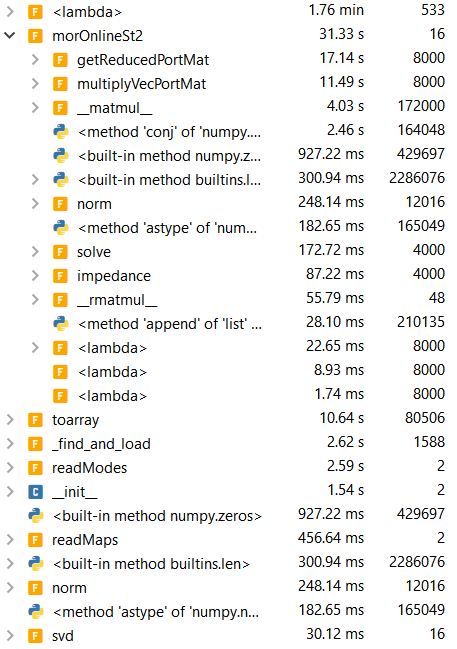
\includegraphics[width=0.3\textwidth]{runtimes_1.PNG}
 	\caption{The total runtime of adaptive version. The meanings are:\\ 1, lambda, reading the data from the drive, mainly the right hand sides;\\ 2. morOnline, the major part of the code; \\2.1+2.2, obviously the major parts of the runtime comes from operations involving the ports. This first due to the large number of calls (8 000) and their subfunctions (80 000), second, because in each call a sparse vector is cast into a dense one, and third, because surprisingly the transpositions are costly. I assume this should be much faster in c++; \\2.3, matmul, part of 2.2;\\ 3, toarray, part of 2.1;\\ svd: calculating the svds is super cheap, just 30ms in total.}
 	\label{fig:st2_sqc_runtime1}
 \end{figure}

\newpage
.
\newpage
\subsubsection{thoughts about stage3}
Stage3 consists of the affine decomposition of the rhs. This serves the reason to calculate the residual faster. In python this may reduce the computational cost quite much, since it would make the calls of multiplyVecPortMat obsolete, which take up 11.5s of the total online time of 31s in Fig.\ref{fig:st2_sqc_runtime1}. A good part (6s) of this  task are transpositions, which should not be costly in c++ . At this point, I assume that the residual computation should not be that costly anyways. Especially if only the beam is used as excitation the sparsity of the RHS could be exploited in the products, instead of searching for an affine decomposition.\\

update: The transpositions are basically free now, since they can be precomputed. Now the large number of matrix vector multiplications in the port-mode functions are the most costly, but this should be cheap in c++. Another expensive task is the computation of gamma, since the root has to be calculated. This could also be solved by precomputations.


\newpage
\subsubsection{Resistive Square Cavity}
The entire surface has an impedance of 5.8e3, so the Sibc matrix comes in affine form.  The convergence is about the same as for the PEC case.


\begin{figure}[h]
	\centering
	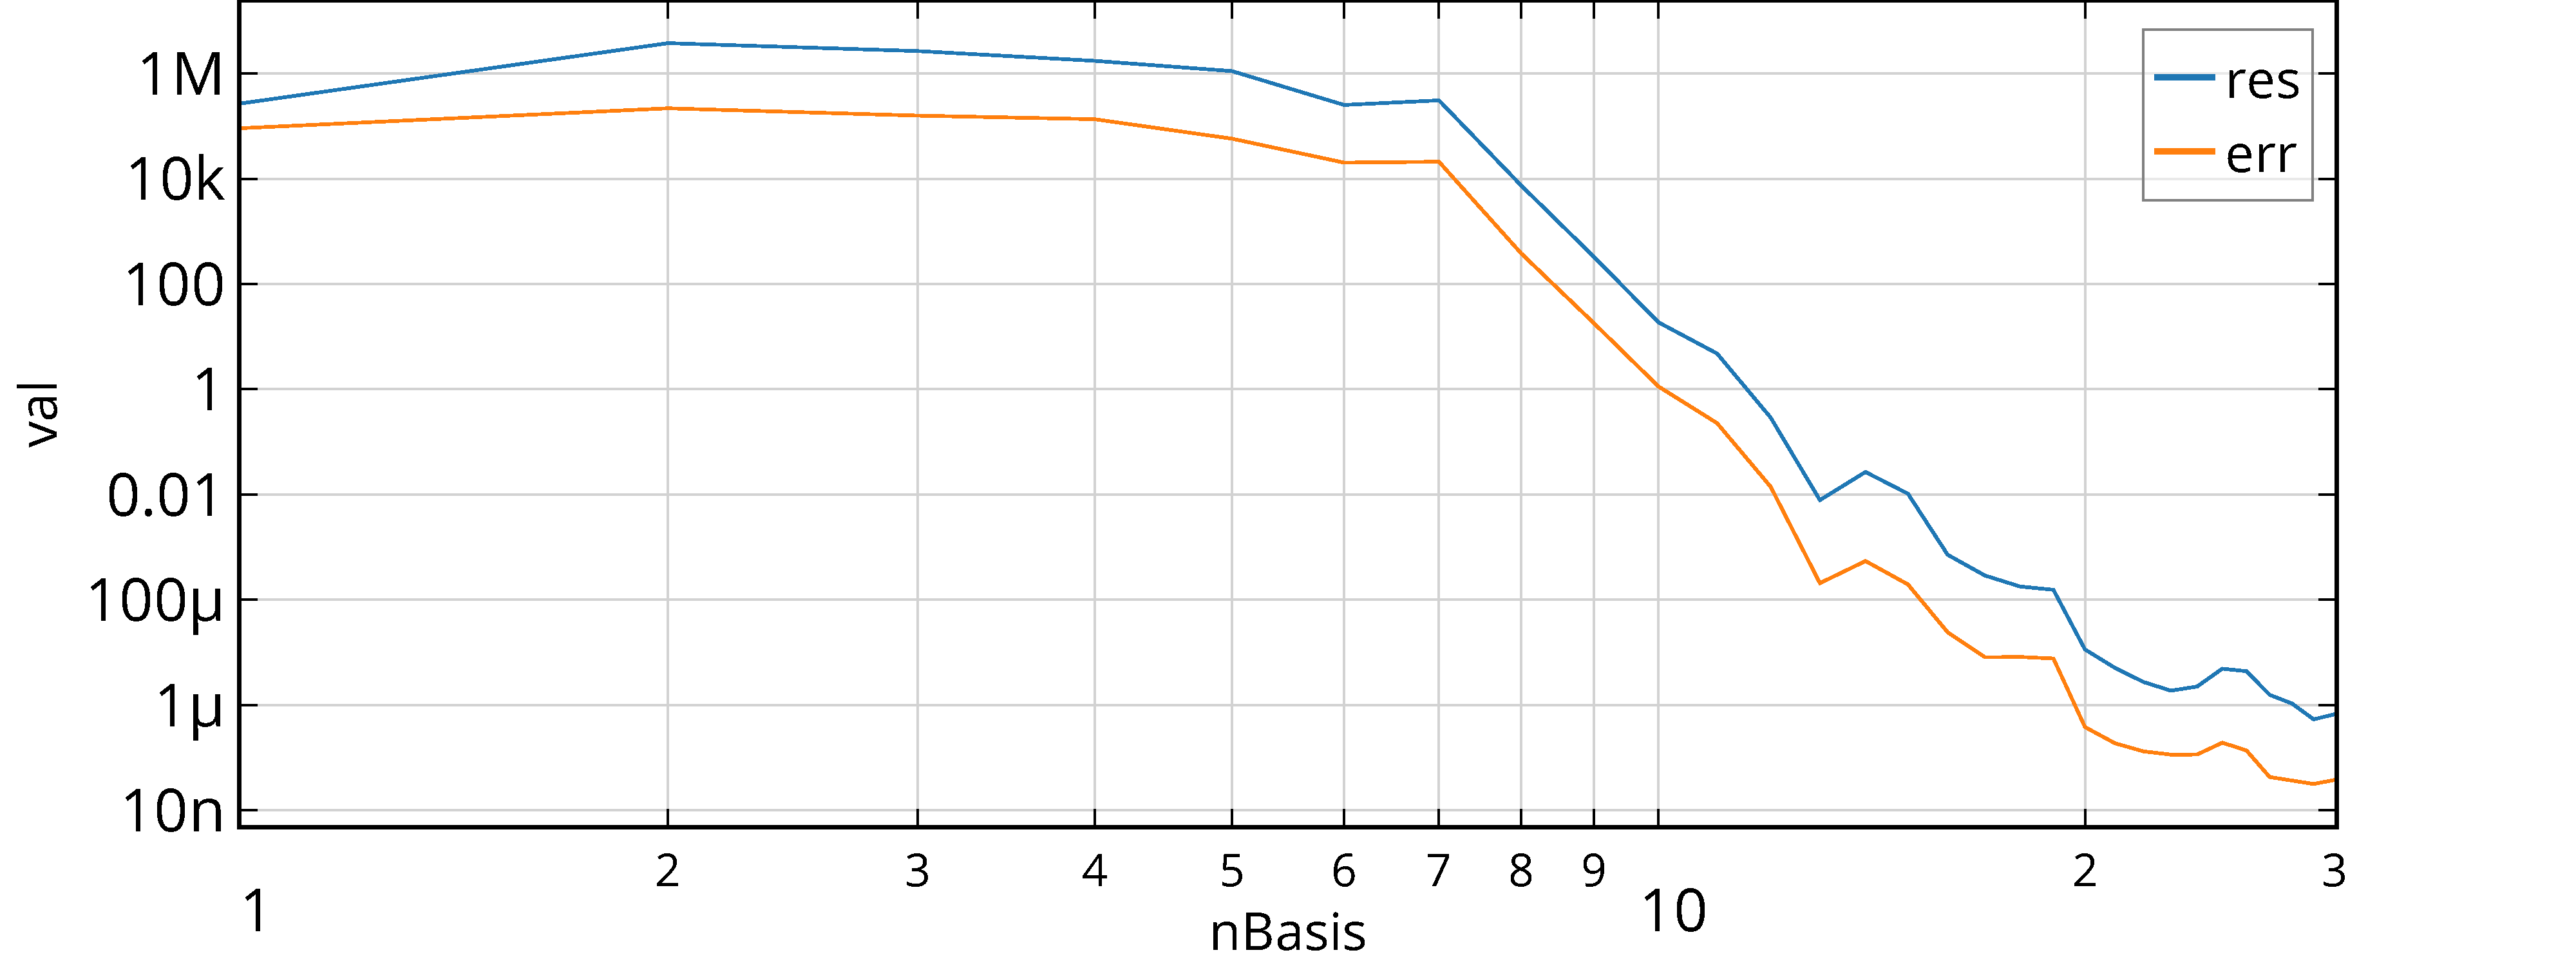
\includegraphics[width=0.5\textwidth]{sqcR_conv_st2_1.pdf}
	\caption{Convergence for the resistive square cavity with linearly spaced points.}
	\label{}
\end{figure}

\begin{figure}[h]
	\centering
	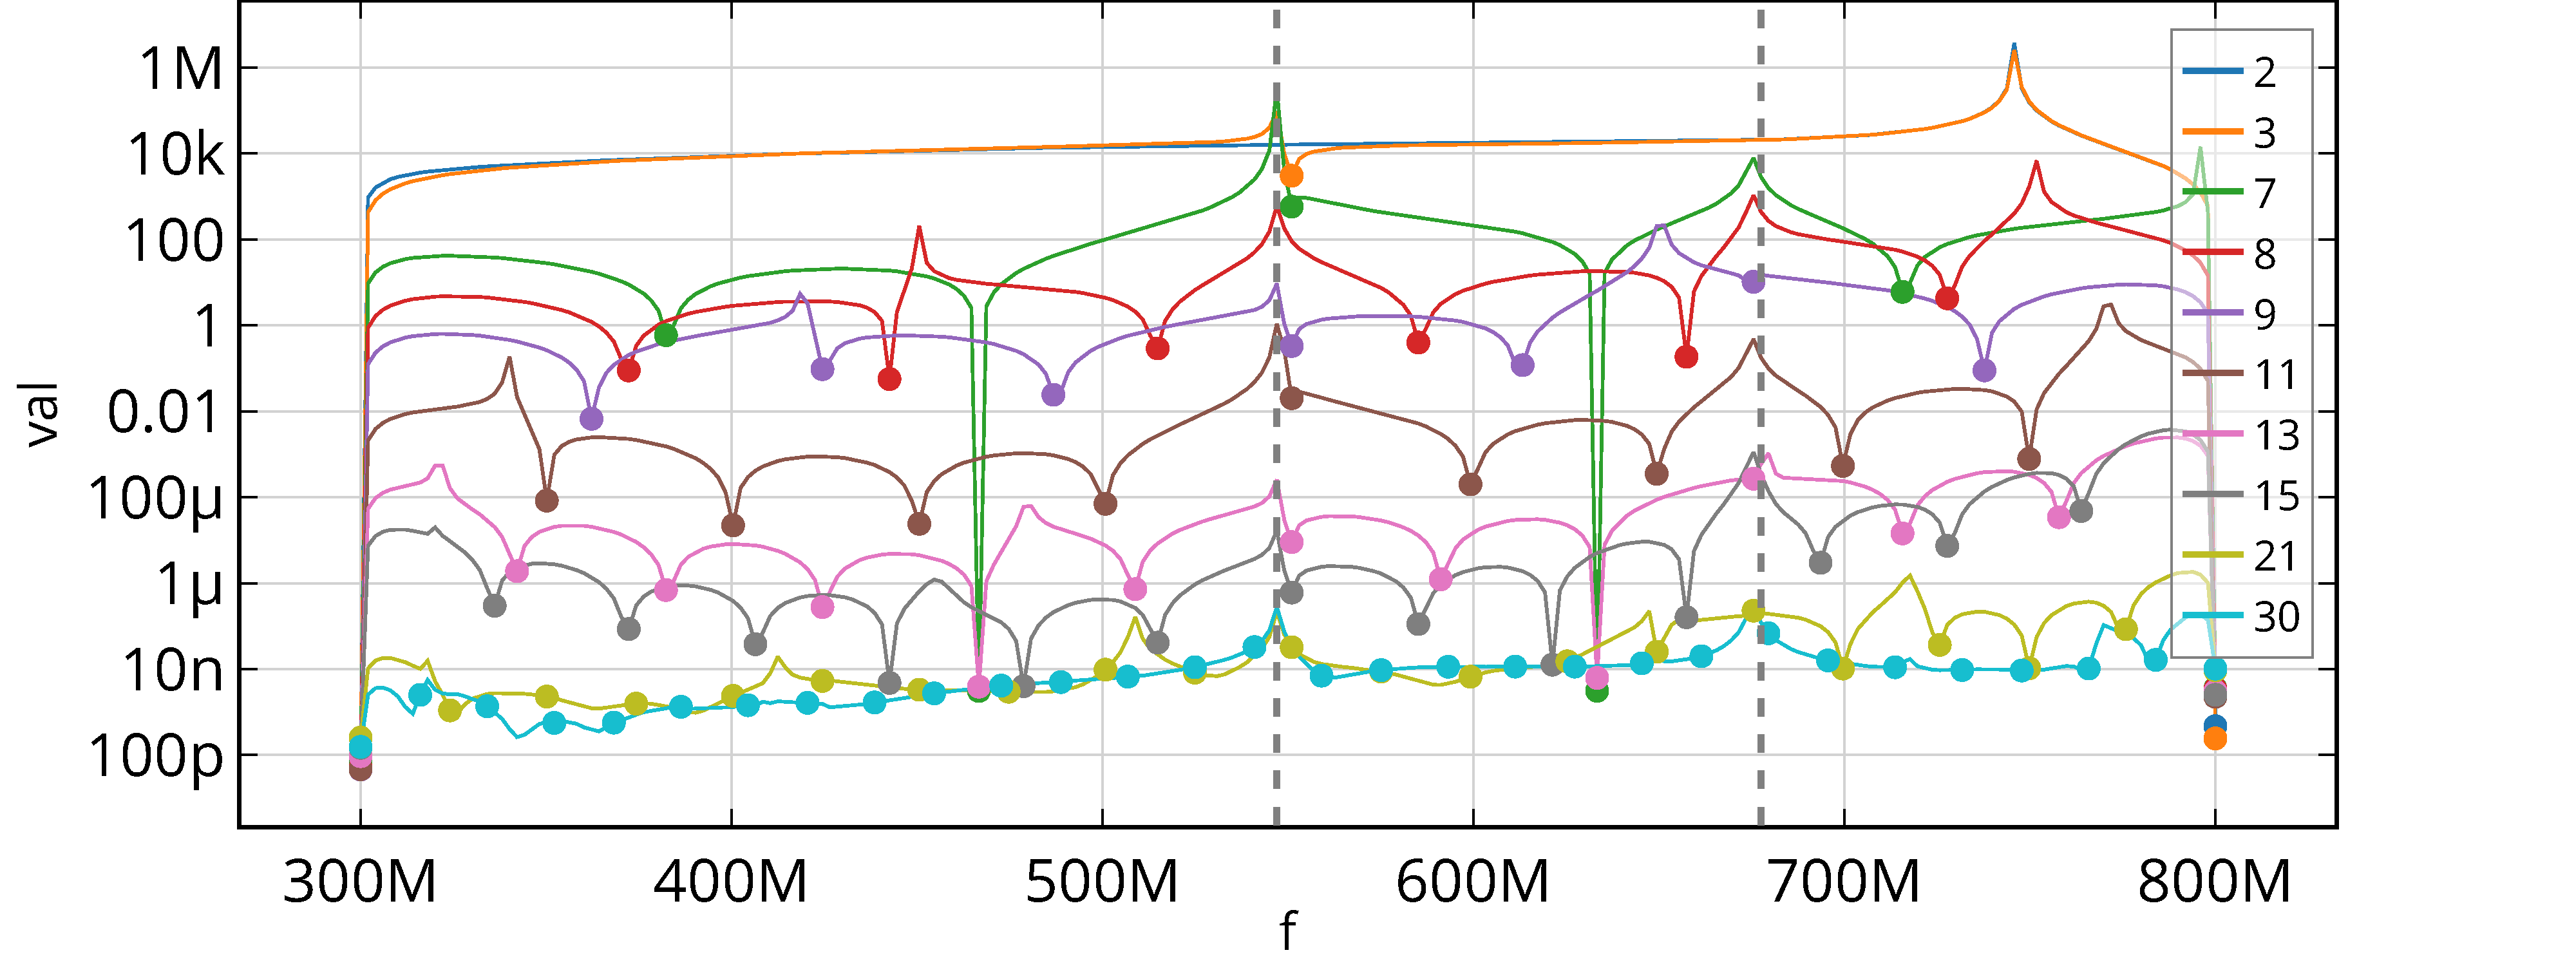
\includegraphics[width=0.5\textwidth]{sqcR_conv_st2_2.pdf}
	\caption{Convergence for the resistive square cavity over frequency. }
	\label{}
\end{figure}


\begin{figure}[h]
	\centering
	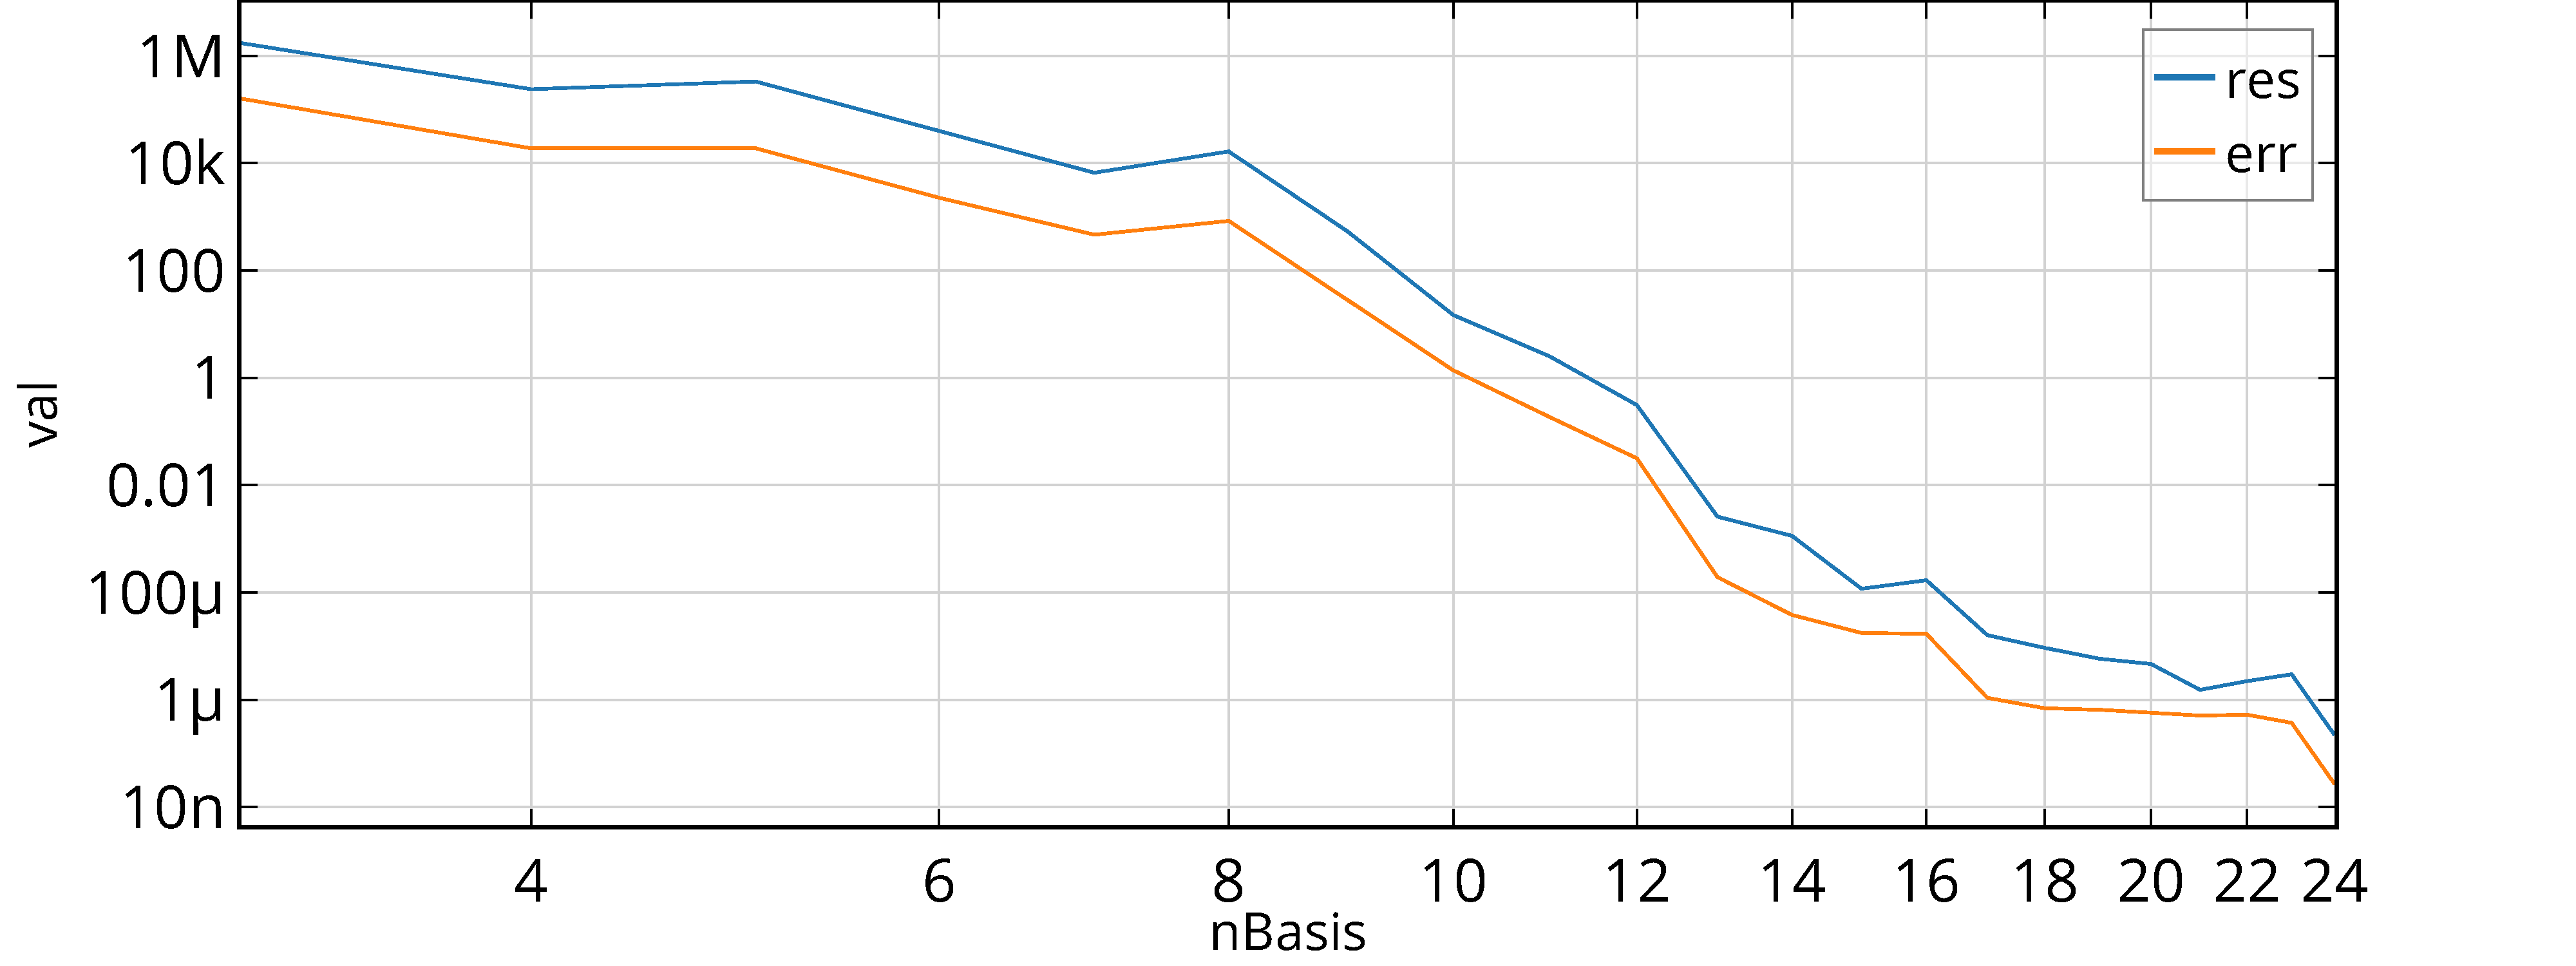
\includegraphics[width=0.5\textwidth]{sqcR_conv_st2_adap_1.pdf}
	\caption{Convergence for the resistive square cavity with adaptive points. The convergence is slightly faster.}
	\label{}
\end{figure}


\newpage.
\subsubsection{Resistive Square Cavity Broadband}
\newpage
\begin{figure}[h]
	\centering
	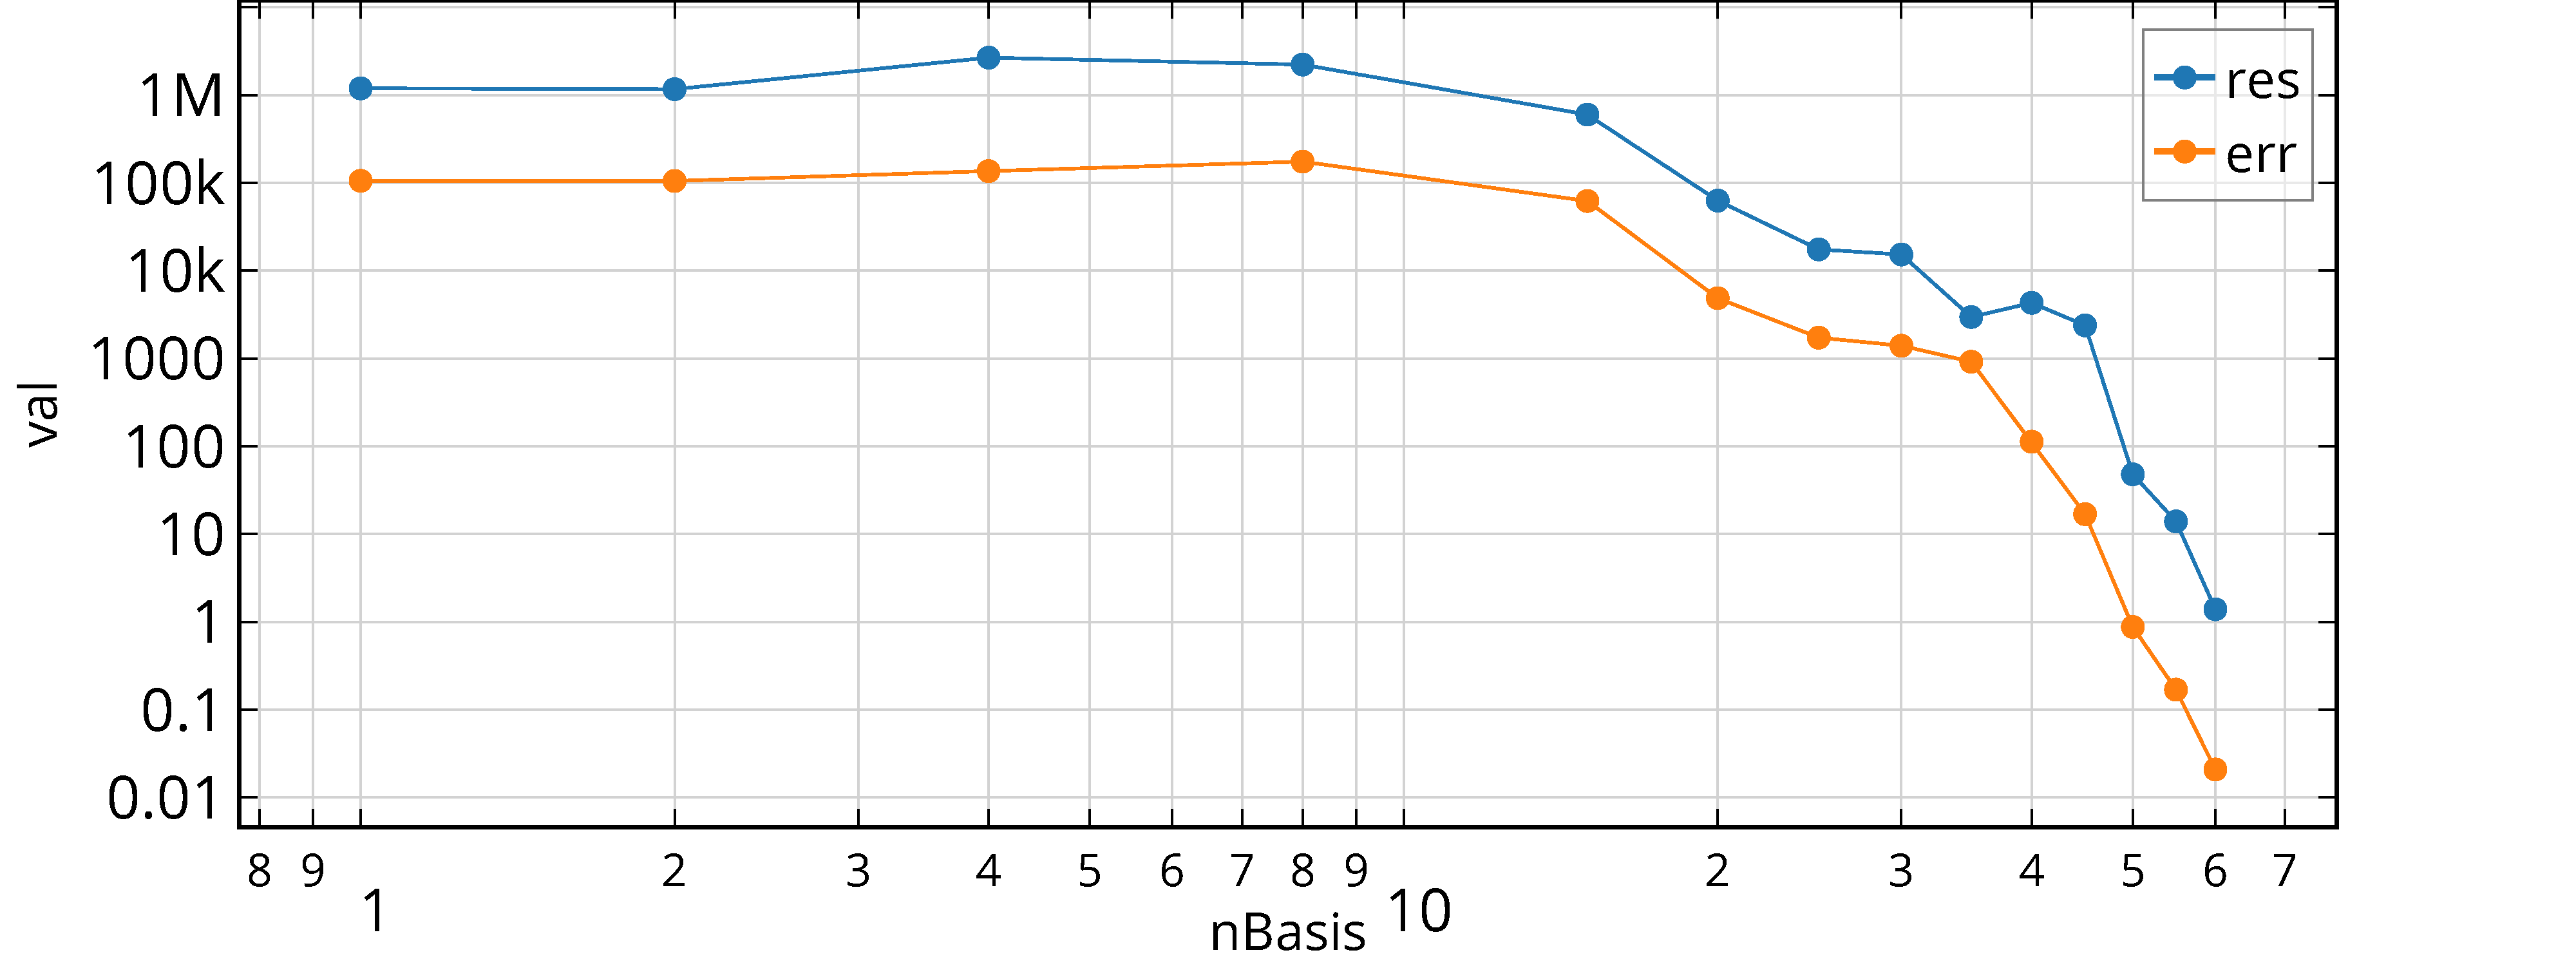
\includegraphics[width=0.5\textwidth]{sqcR_conv_st2_broad1.pdf}
	\caption{Convergence for the resistive square cavity with linearly spaced points over a broad frequency range.}
	\label{}
\end{figure}

\begin{figure}[h]
	\centering
	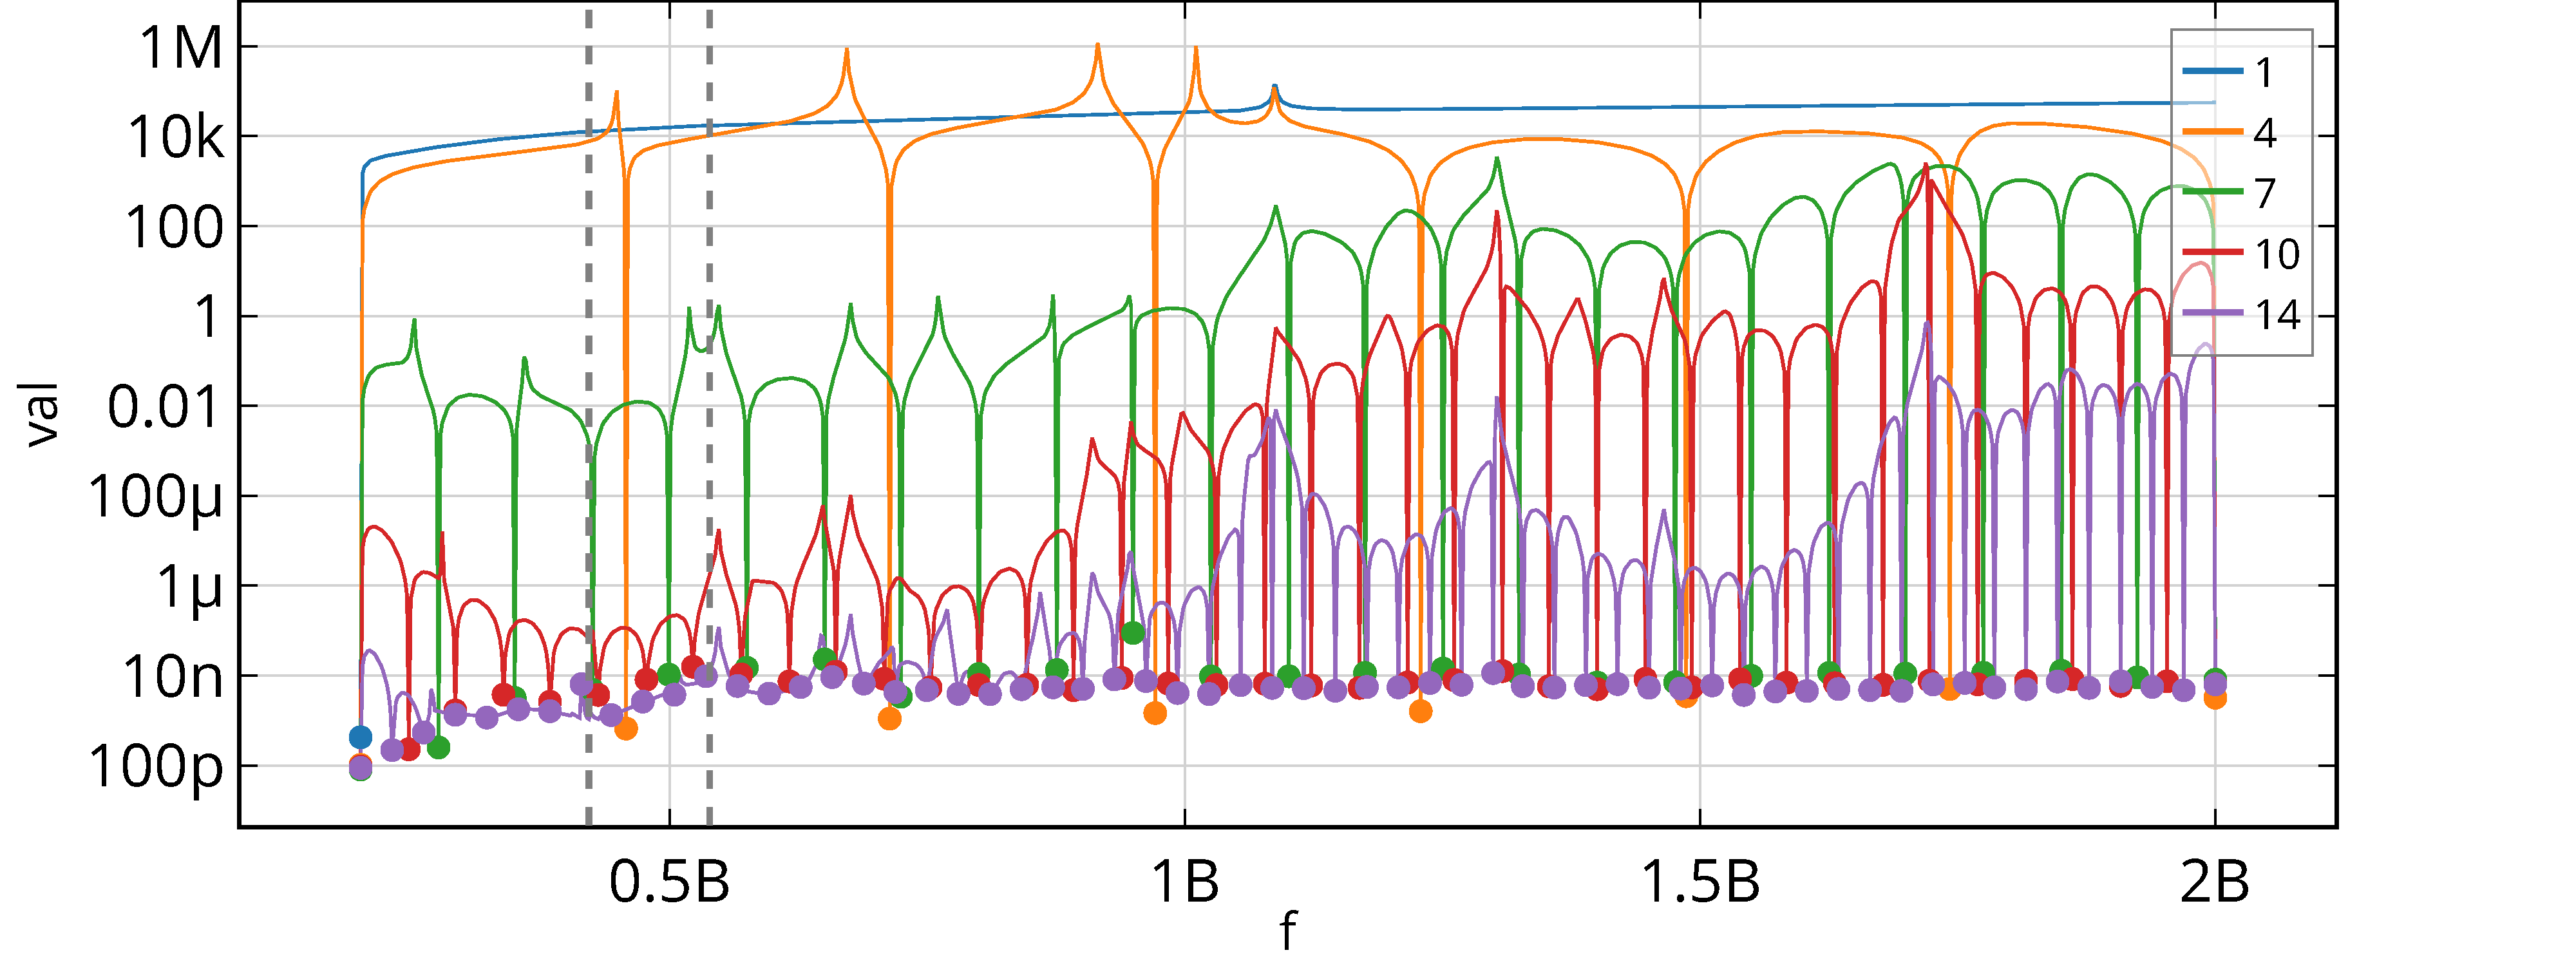
\includegraphics[width=0.5\textwidth]{sqcR_conv_st2_broad2.pdf}
	\caption{Convergence for the resistive square cavity over frequency. Compared to the previous examples, this time the convergence is not uniform and significantly quicker in the lower frequencies. The numbers don't equal the number of basis functions: 14=60}
	\label{}
\end{figure}


\begin{figure}[h]
	\centering
	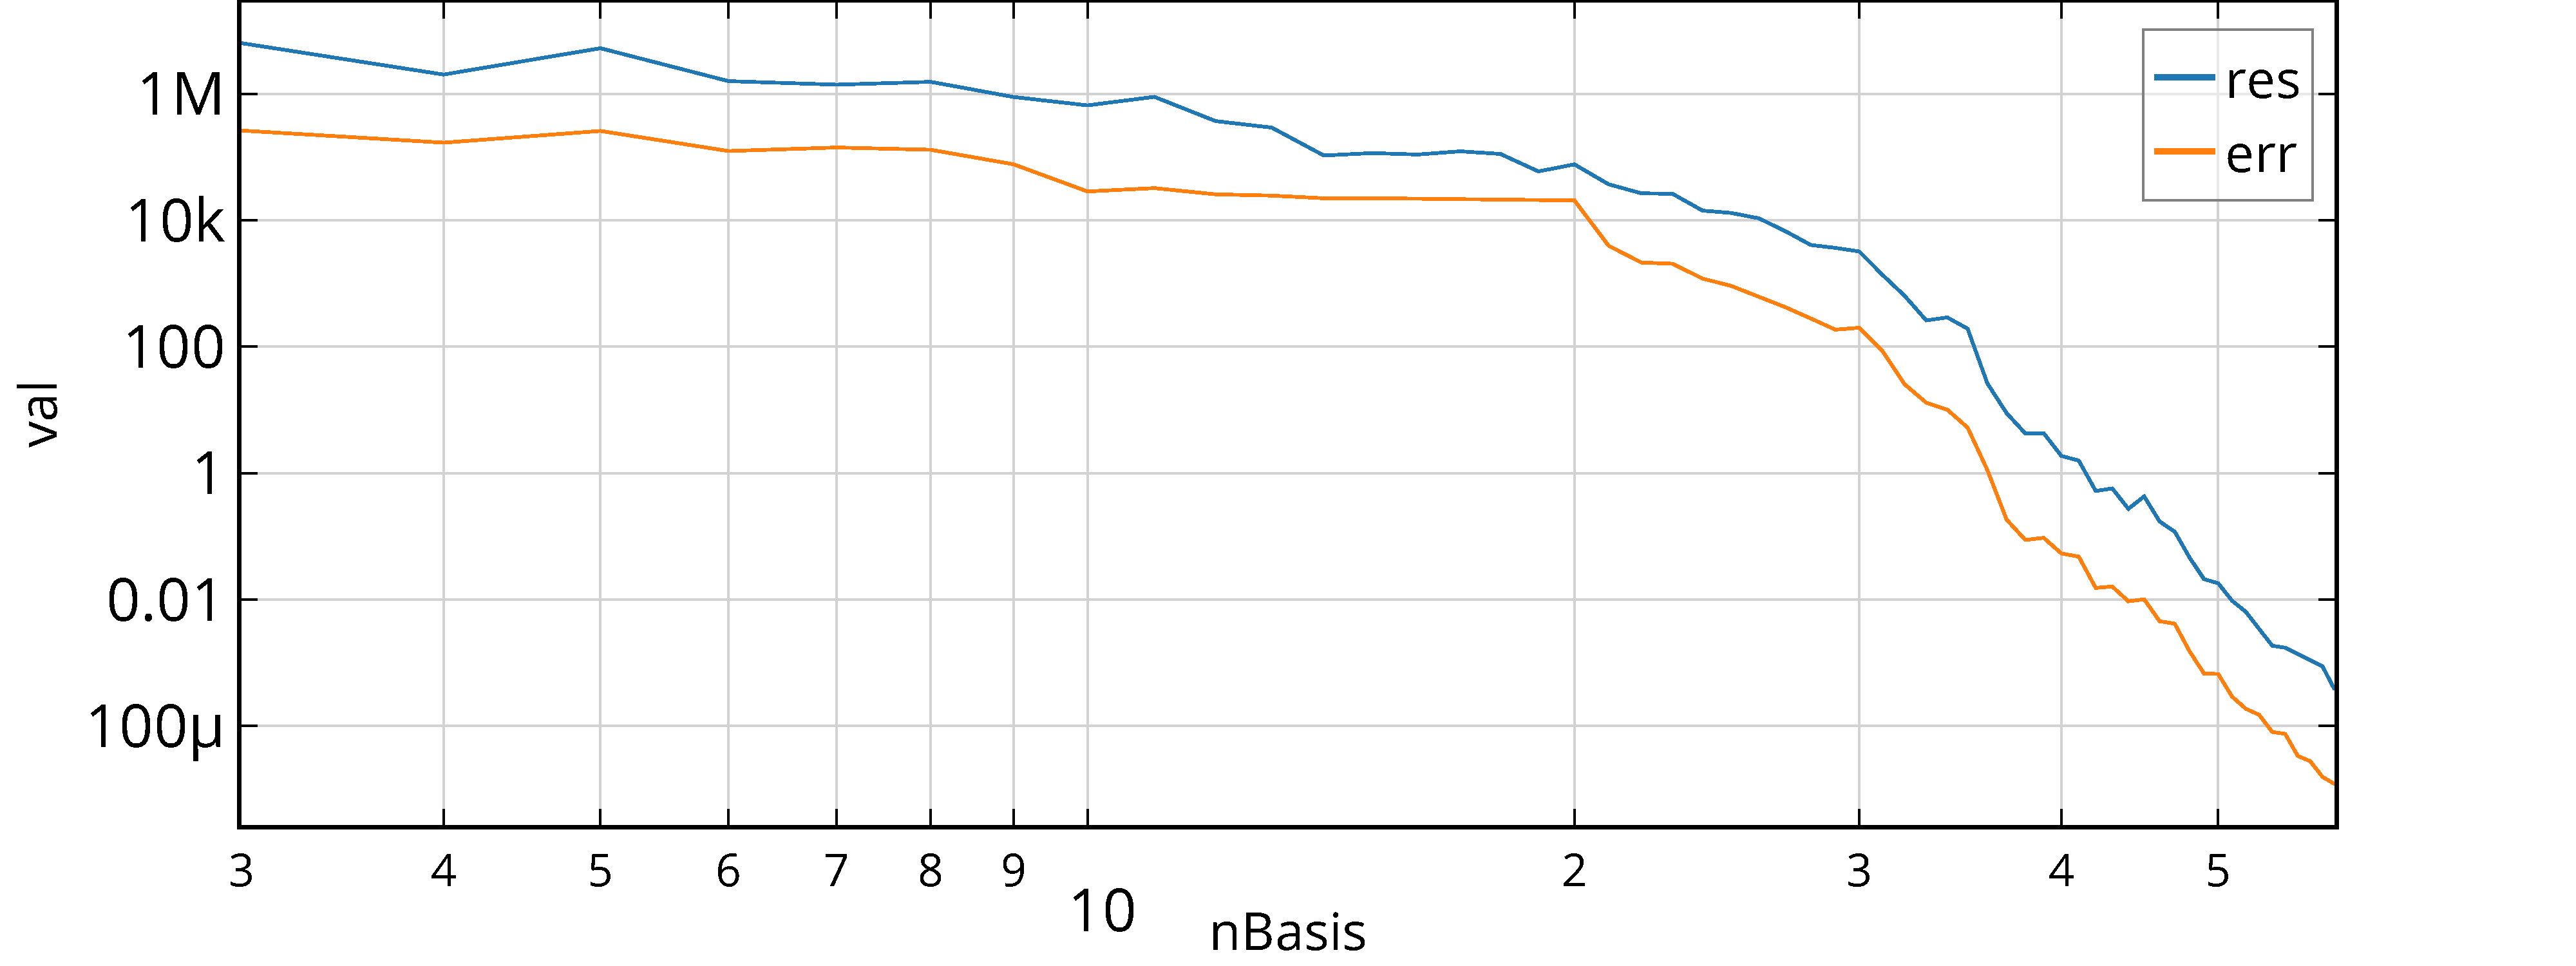
\includegraphics[width=0.5\textwidth]{sqcR_conv_st2_adap_broad1.pdf}
	\caption{Convergence for the resistive square cavity with adaptive  points.}
	\label{}
\end{figure}

\begin{figure}[h]
	\centering
	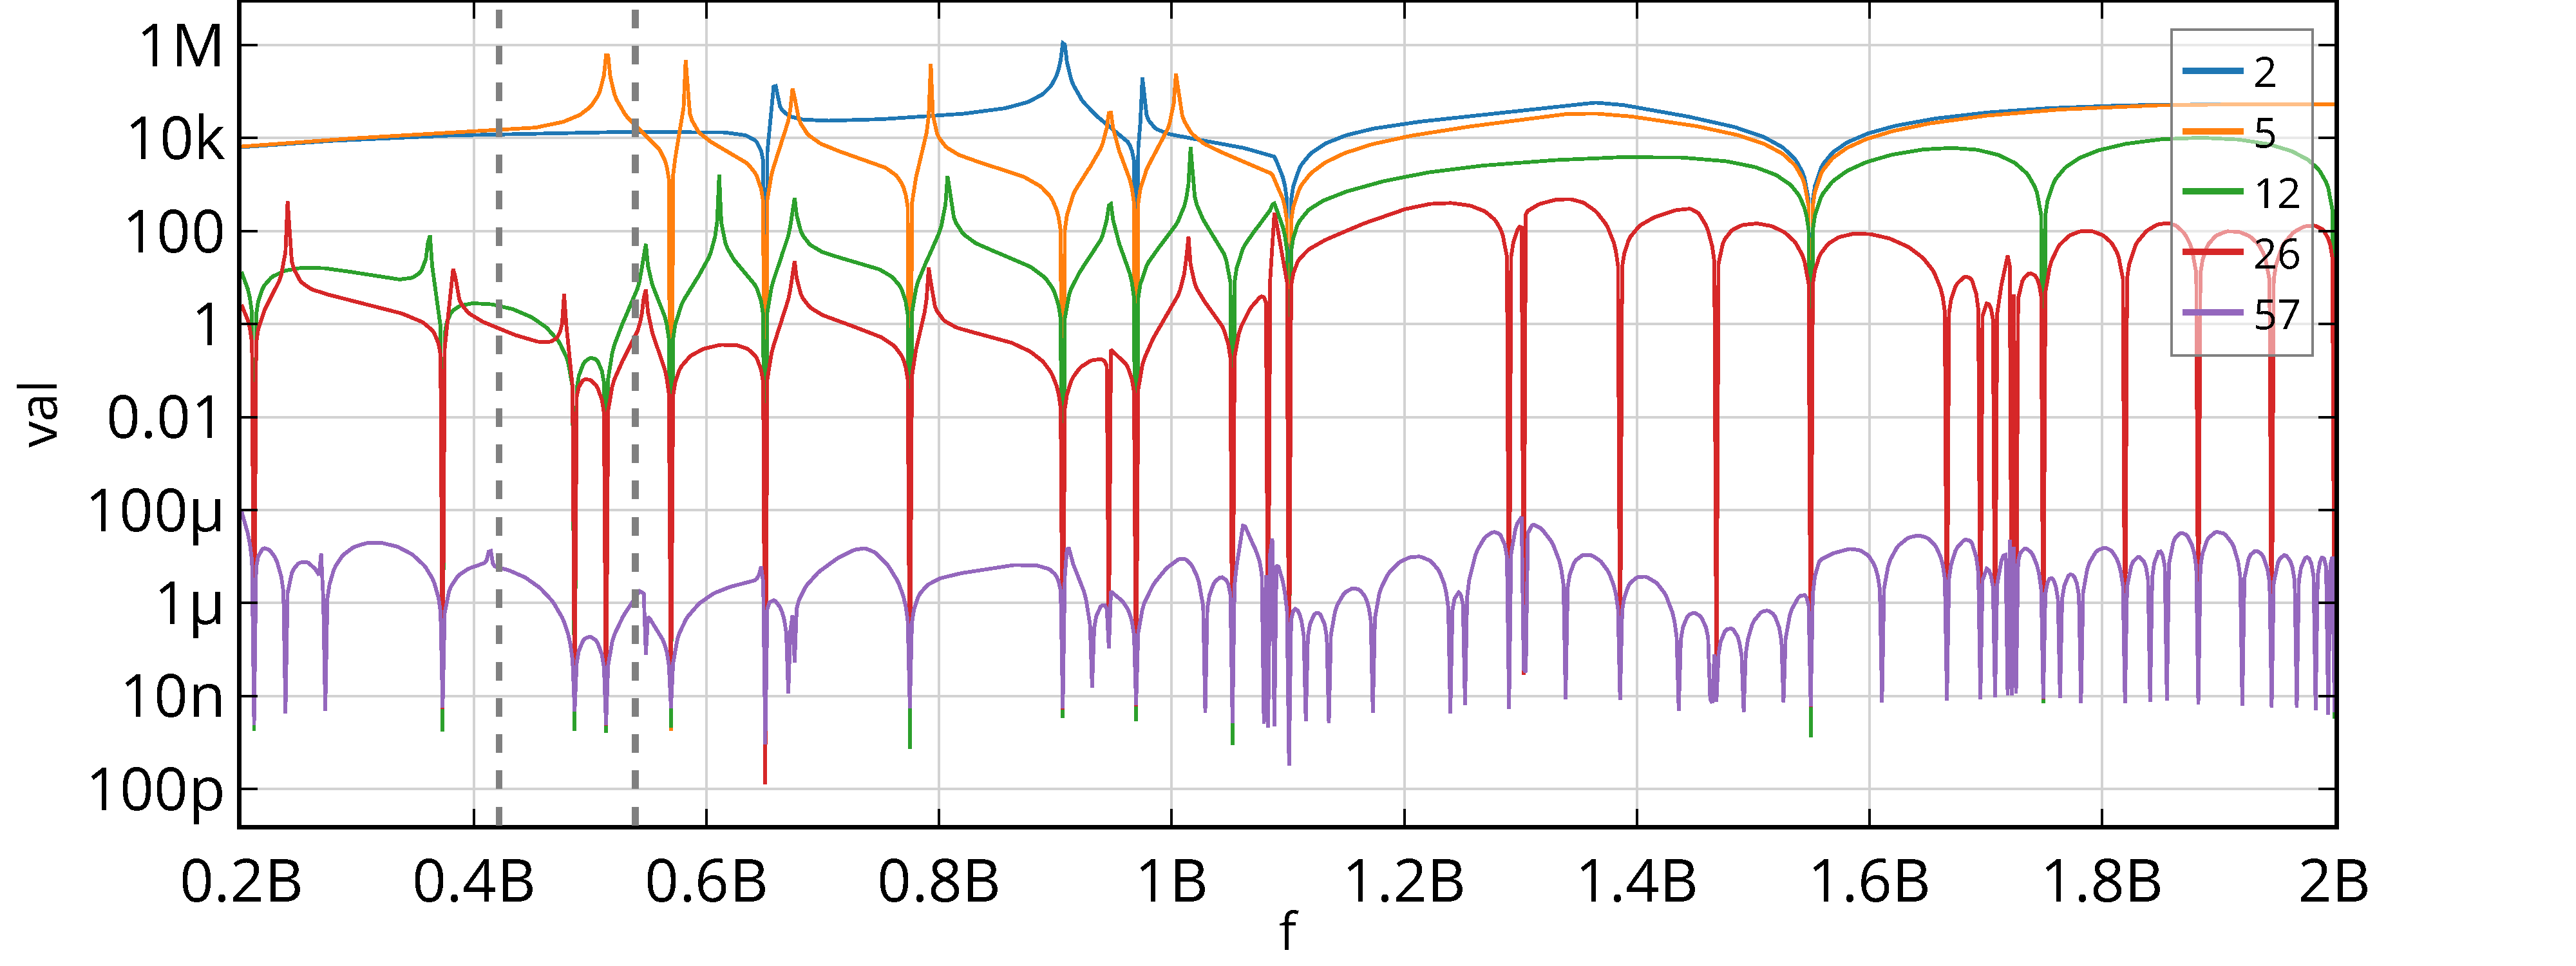
\includegraphics[width=0.5\textwidth]{sqcR_conv_st2_adap_broad2.pdf}
	\caption{Convergence for the resistive square cavity over frequency with adaptive sampling. Compared to the previous example, this time the convergence is uniform.}
	\label{}
\end{figure}

\begin{figure}[h]
	\centering
	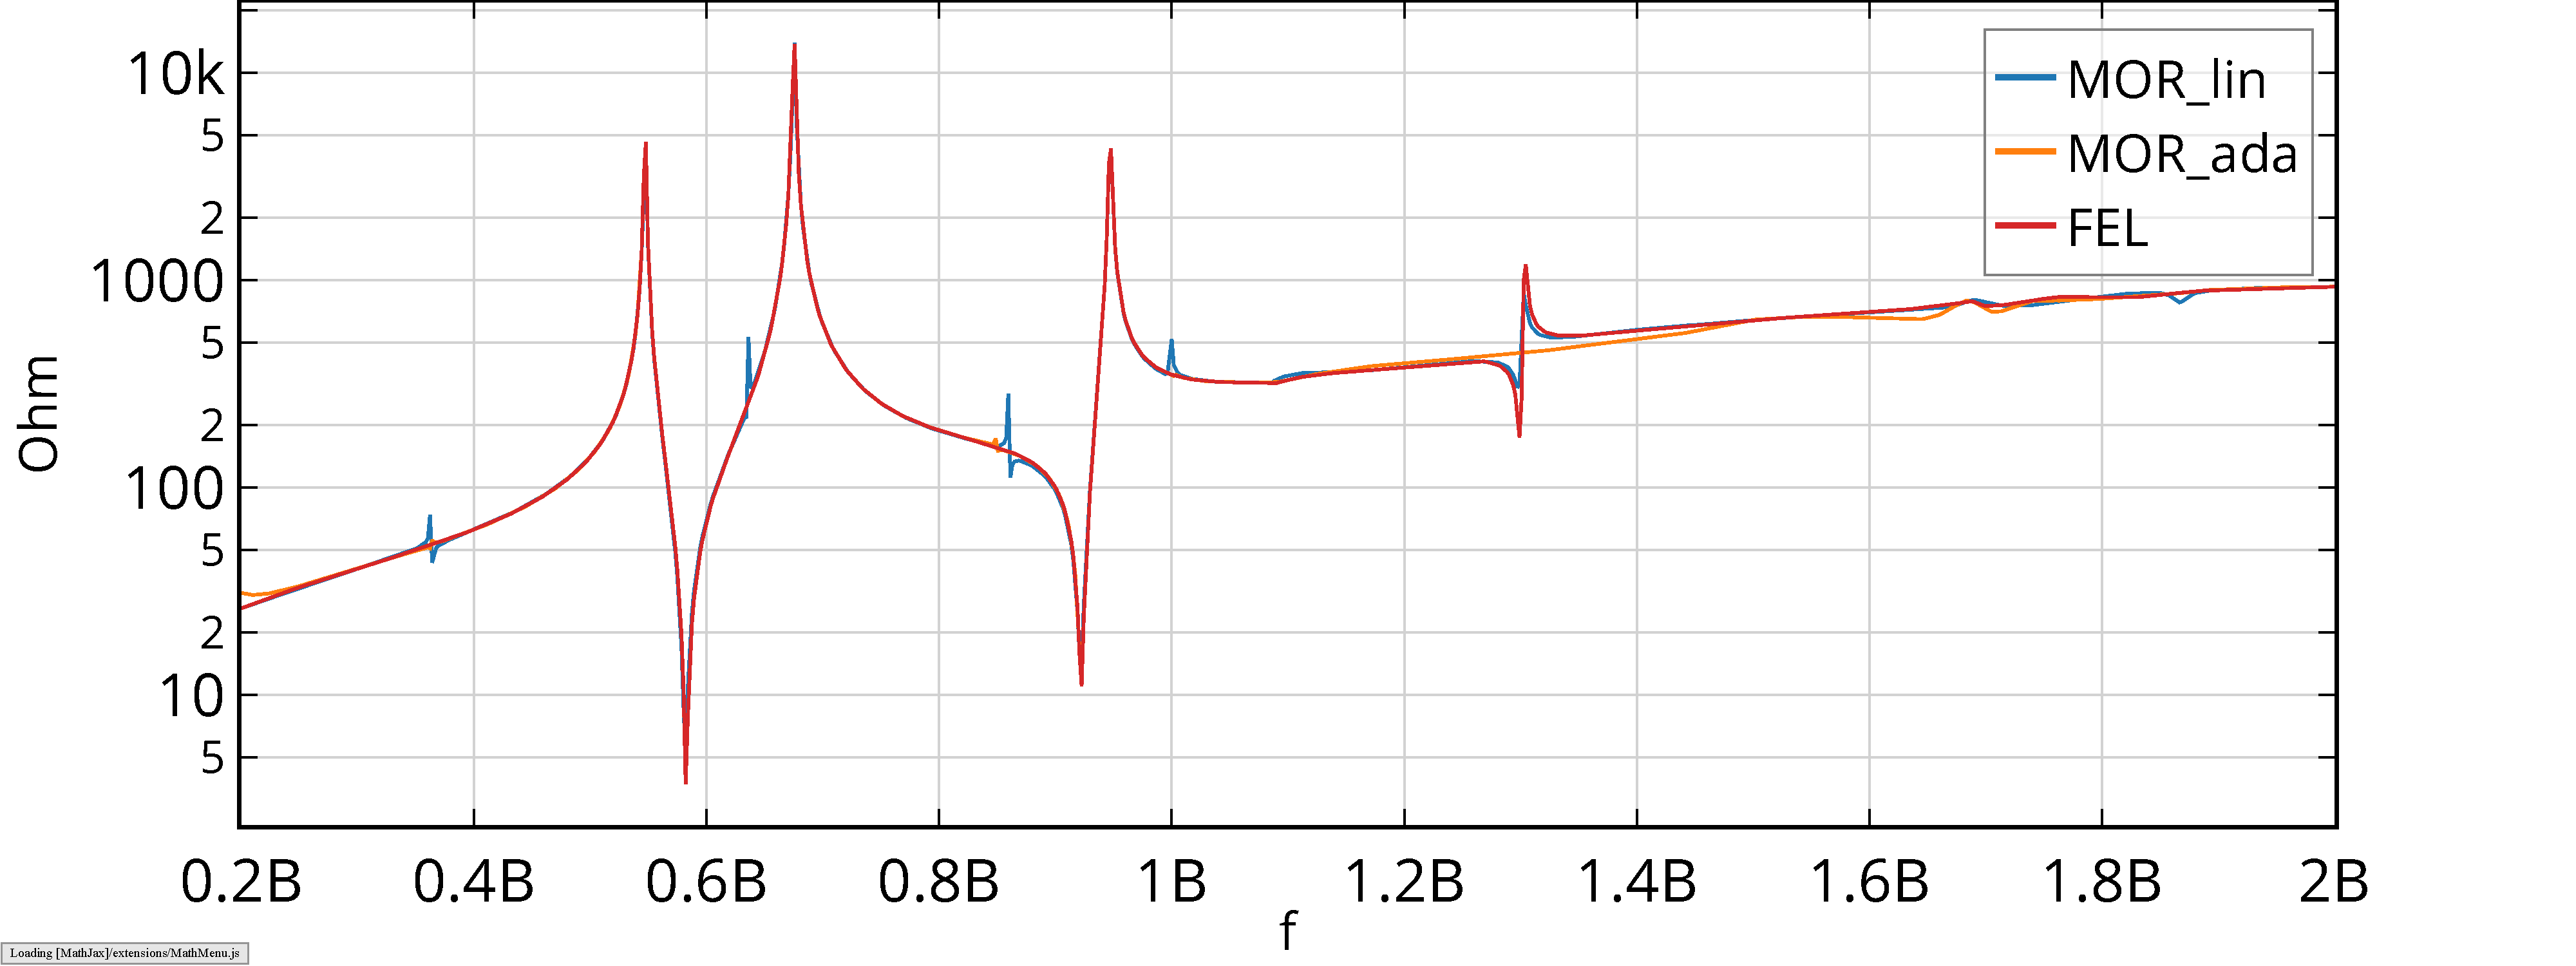
\includegraphics[width=0.5\textwidth]{sqcR_imp_ada1.pdf}
	\caption{Magnitude of the impedance for 18 basis functions. This number is chosen so that some error is visible. It is difficult to say whether the adaptive or non-adaptive version is better. The non-adaptive found all resonances, but has four spurious ones. The adaptive one has no spurious resonances but is missing the last resonance.}
	\label{}
\end{figure}

\newpage.
\subsubsection{Constriction}

%\begin{figure}[h]
%	\centering
%	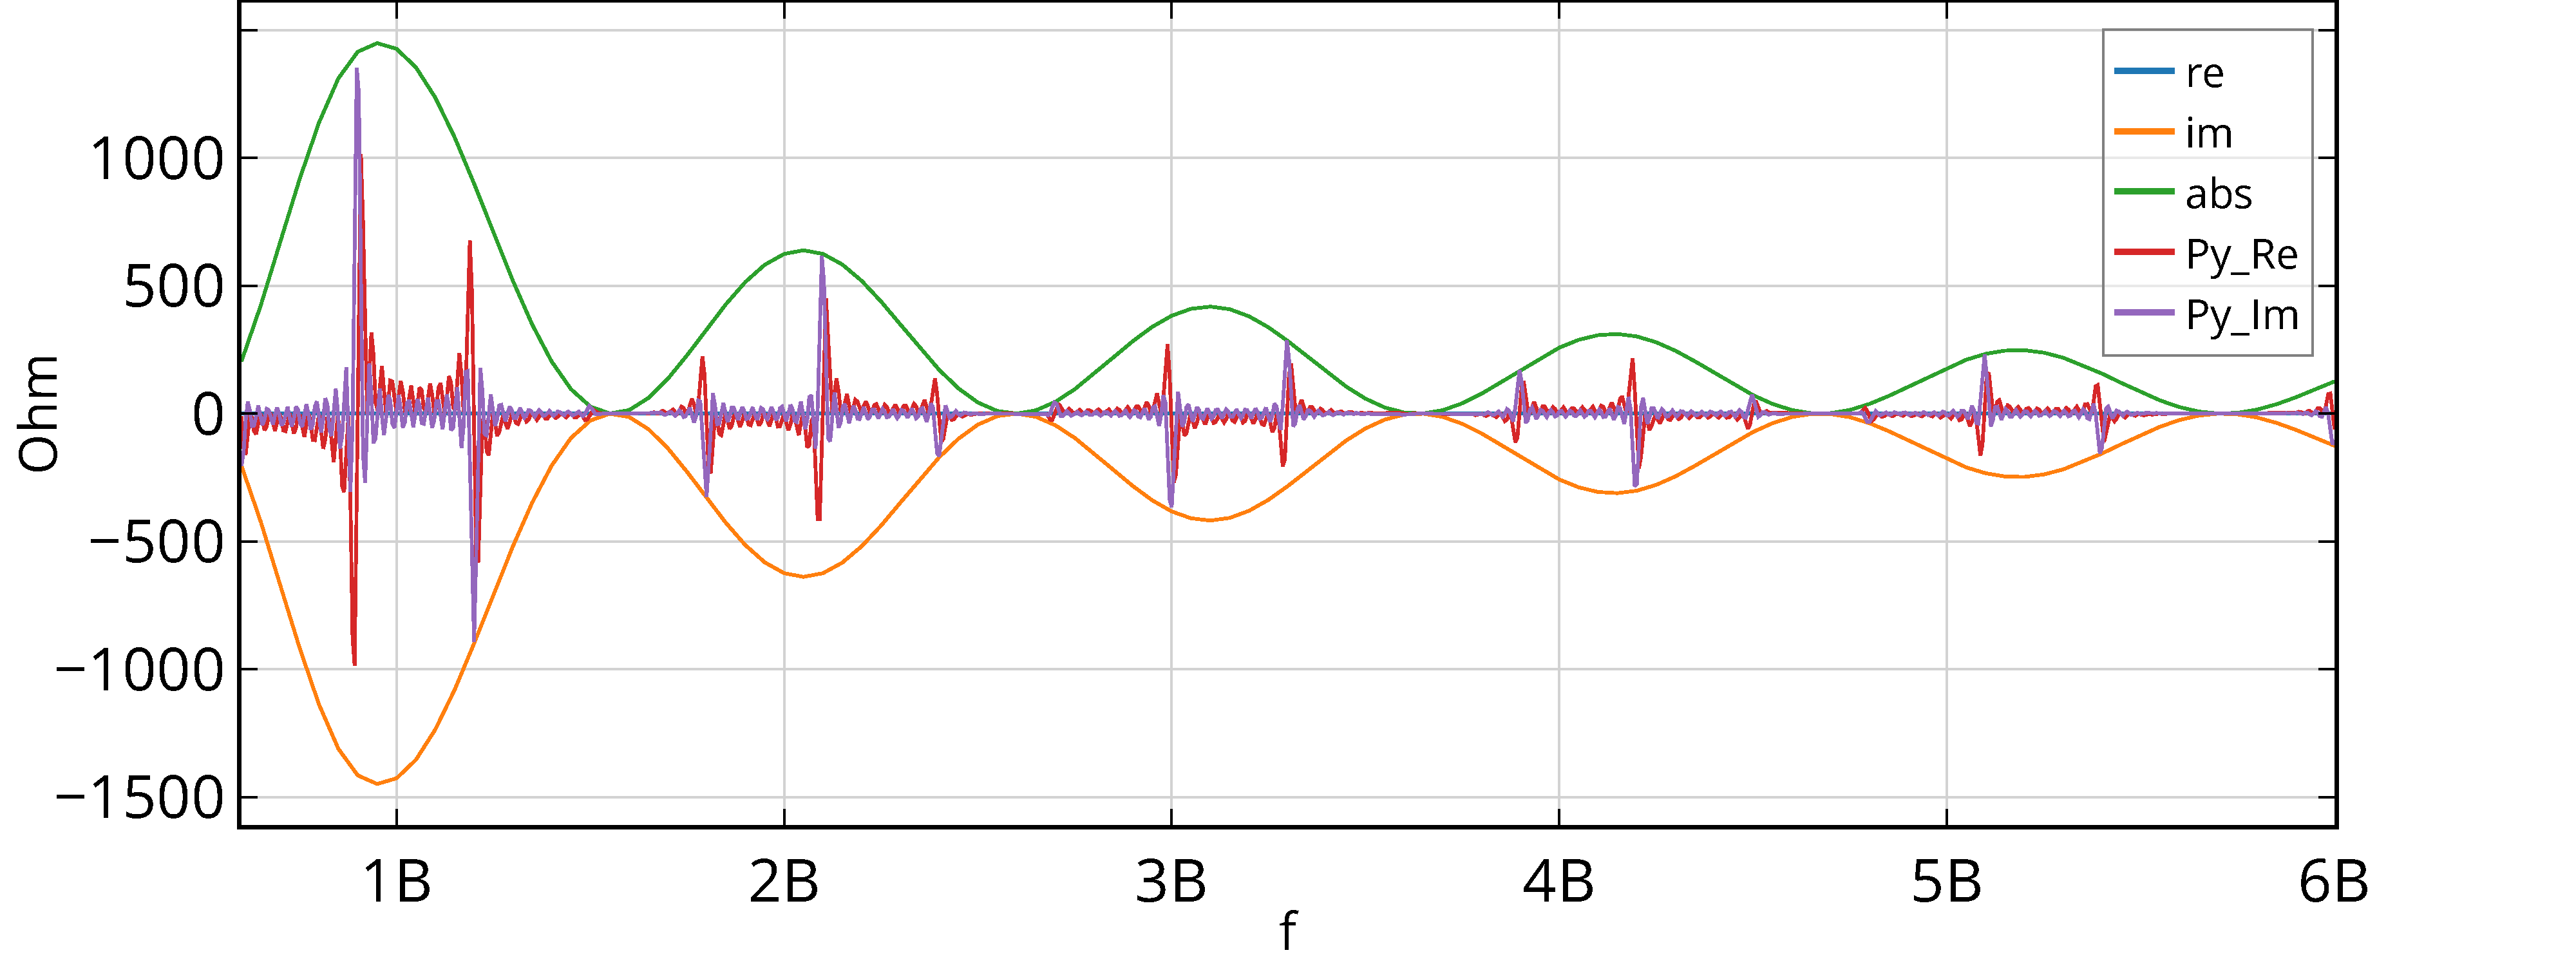
\includegraphics[width=0.5\textwidth]{const_imp_Felis_Py.pdf}
%	\caption{impedances calculated by the post processing in the FELIS code, vs impedances calculated from the field solutions of FELIS by python. The real part of the solution by FELIS is low, around 0.1, vs up to 1500 of the imaginary part. The impedance calculated by the python code is obviously very different...}
%	\label{}
%\end{figure}

\begin{figure}[h]
	\centering
	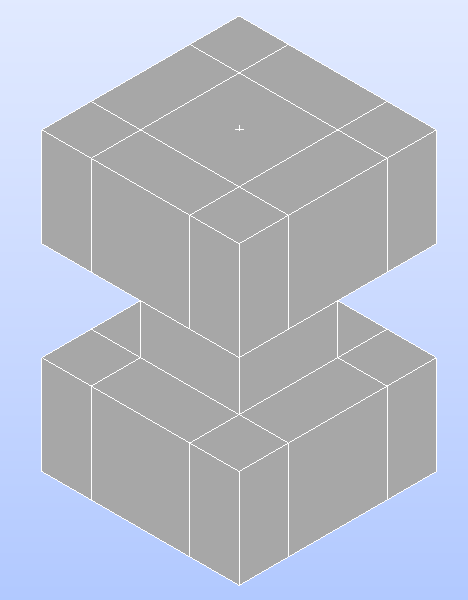
\includegraphics[width=0.5\textwidth]{ConstrictionGeo.PNG}
	\caption{Geometry of the constriction model. Surface impedance=5.8e6 S/m }
	\label{}
\end{figure}

\begin{figure}[h]
	\centering
	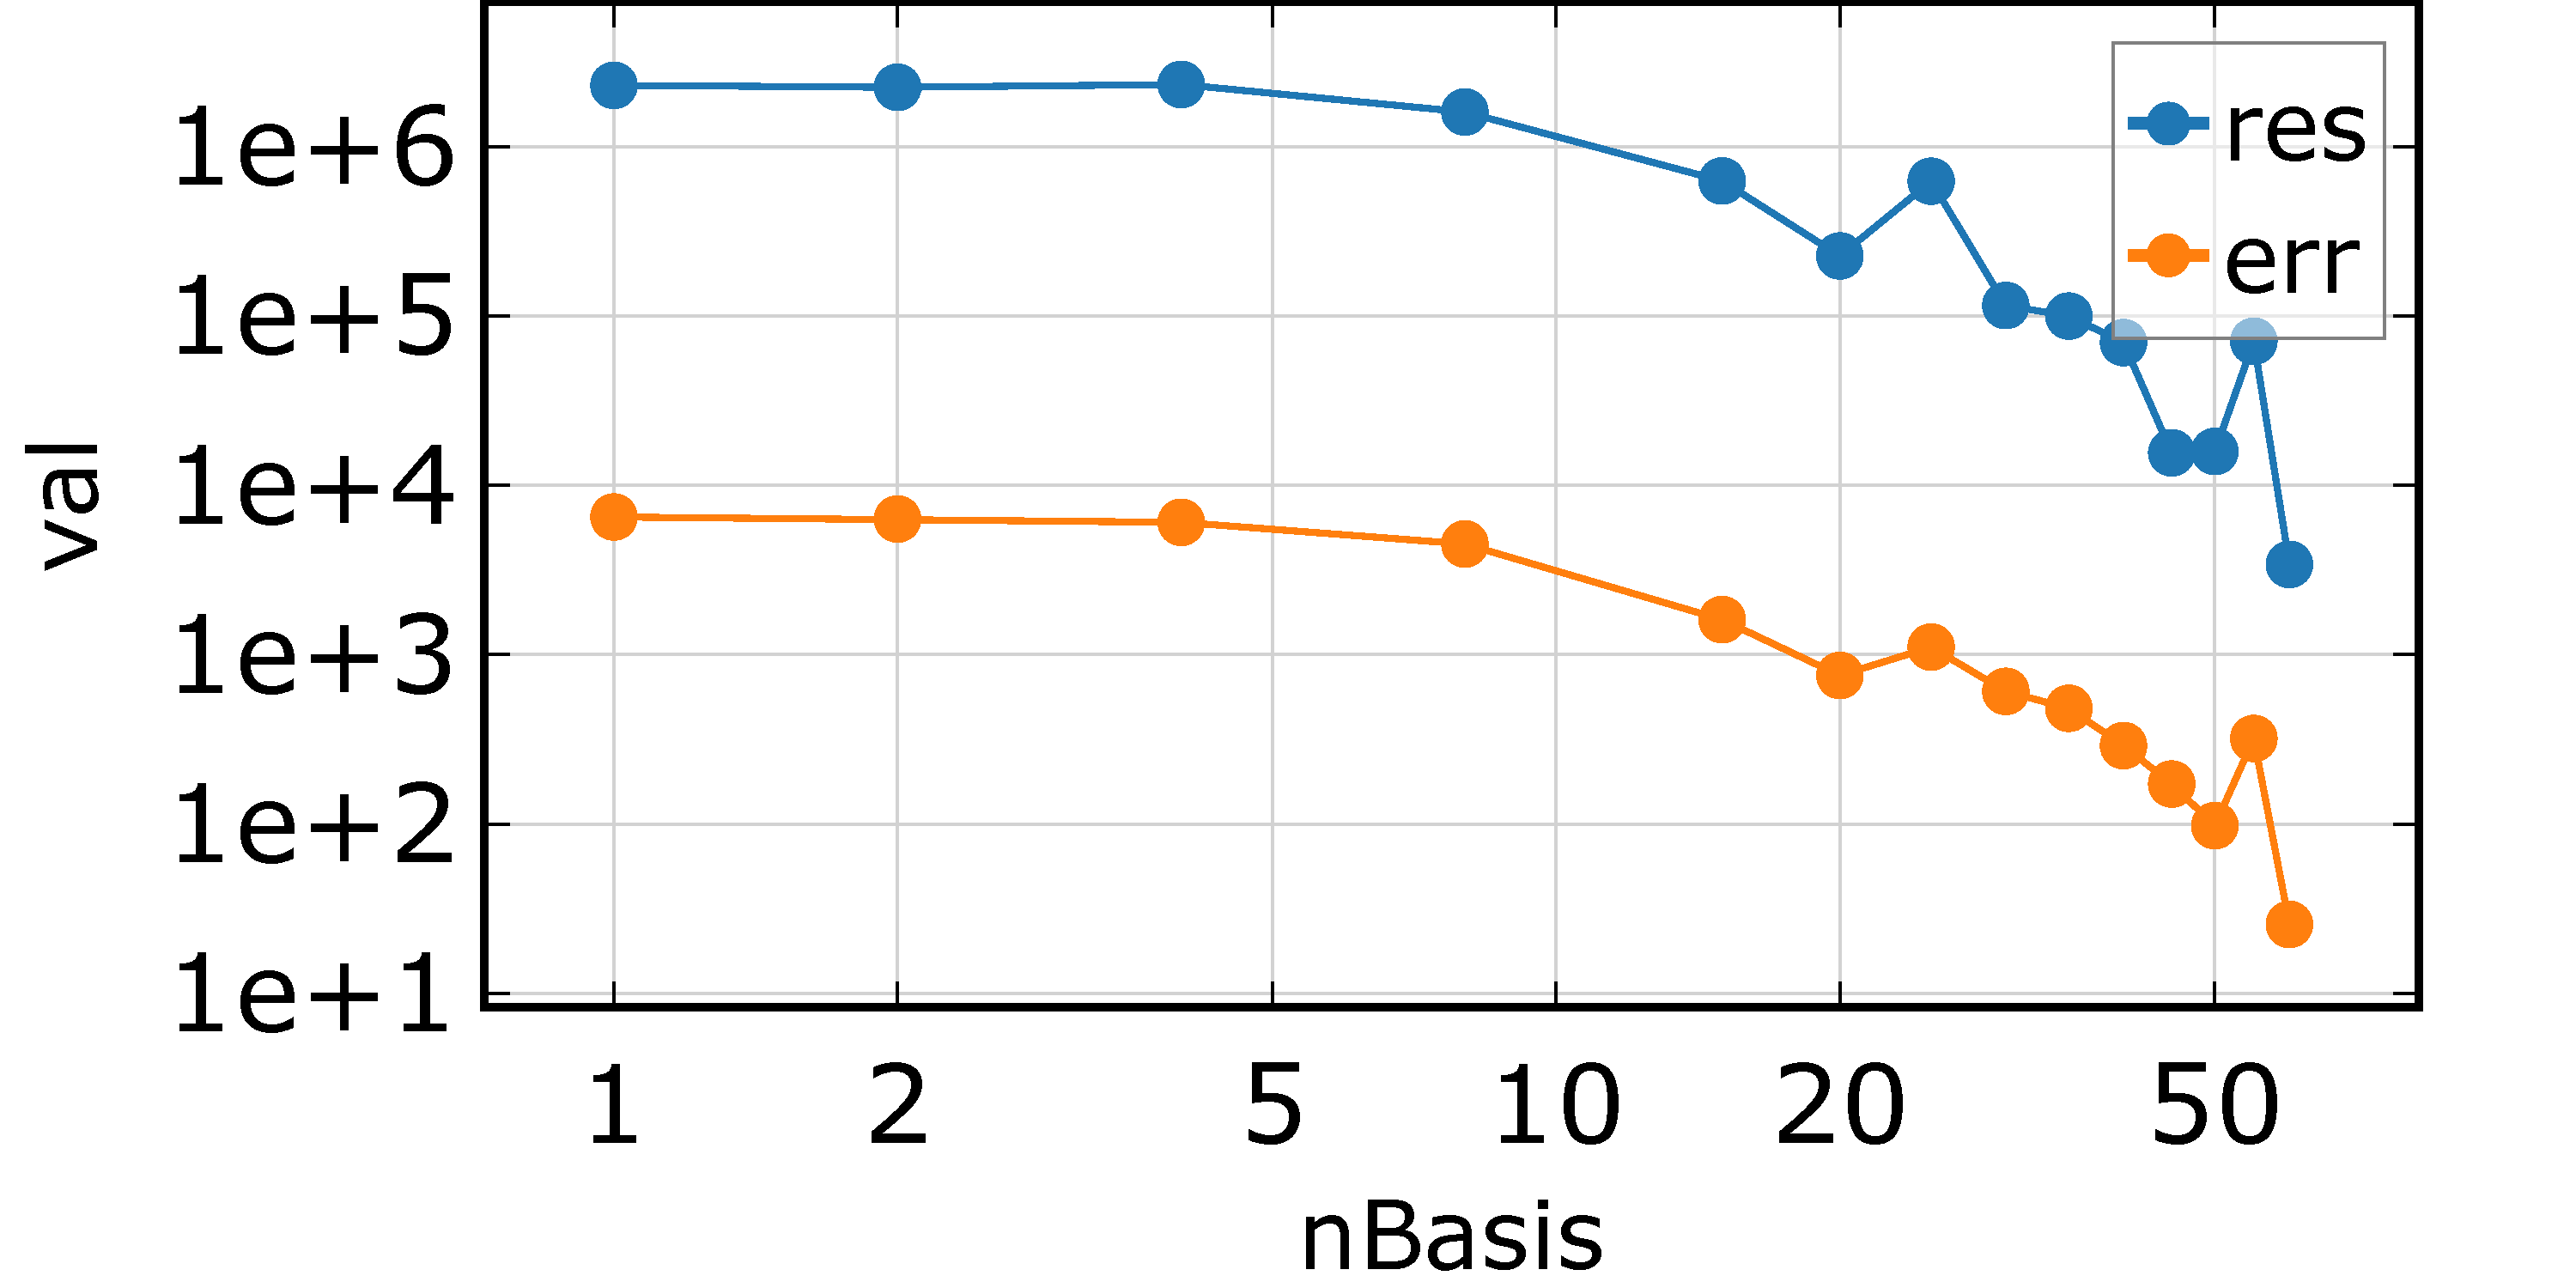
\includegraphics[width=0.5\textwidth]{const_conv_st2_broad1.pdf}
	\caption{Convergence for the non-adaptive code }
	\label{}
\end{figure}


\begin{figure}[h]
	\centering
	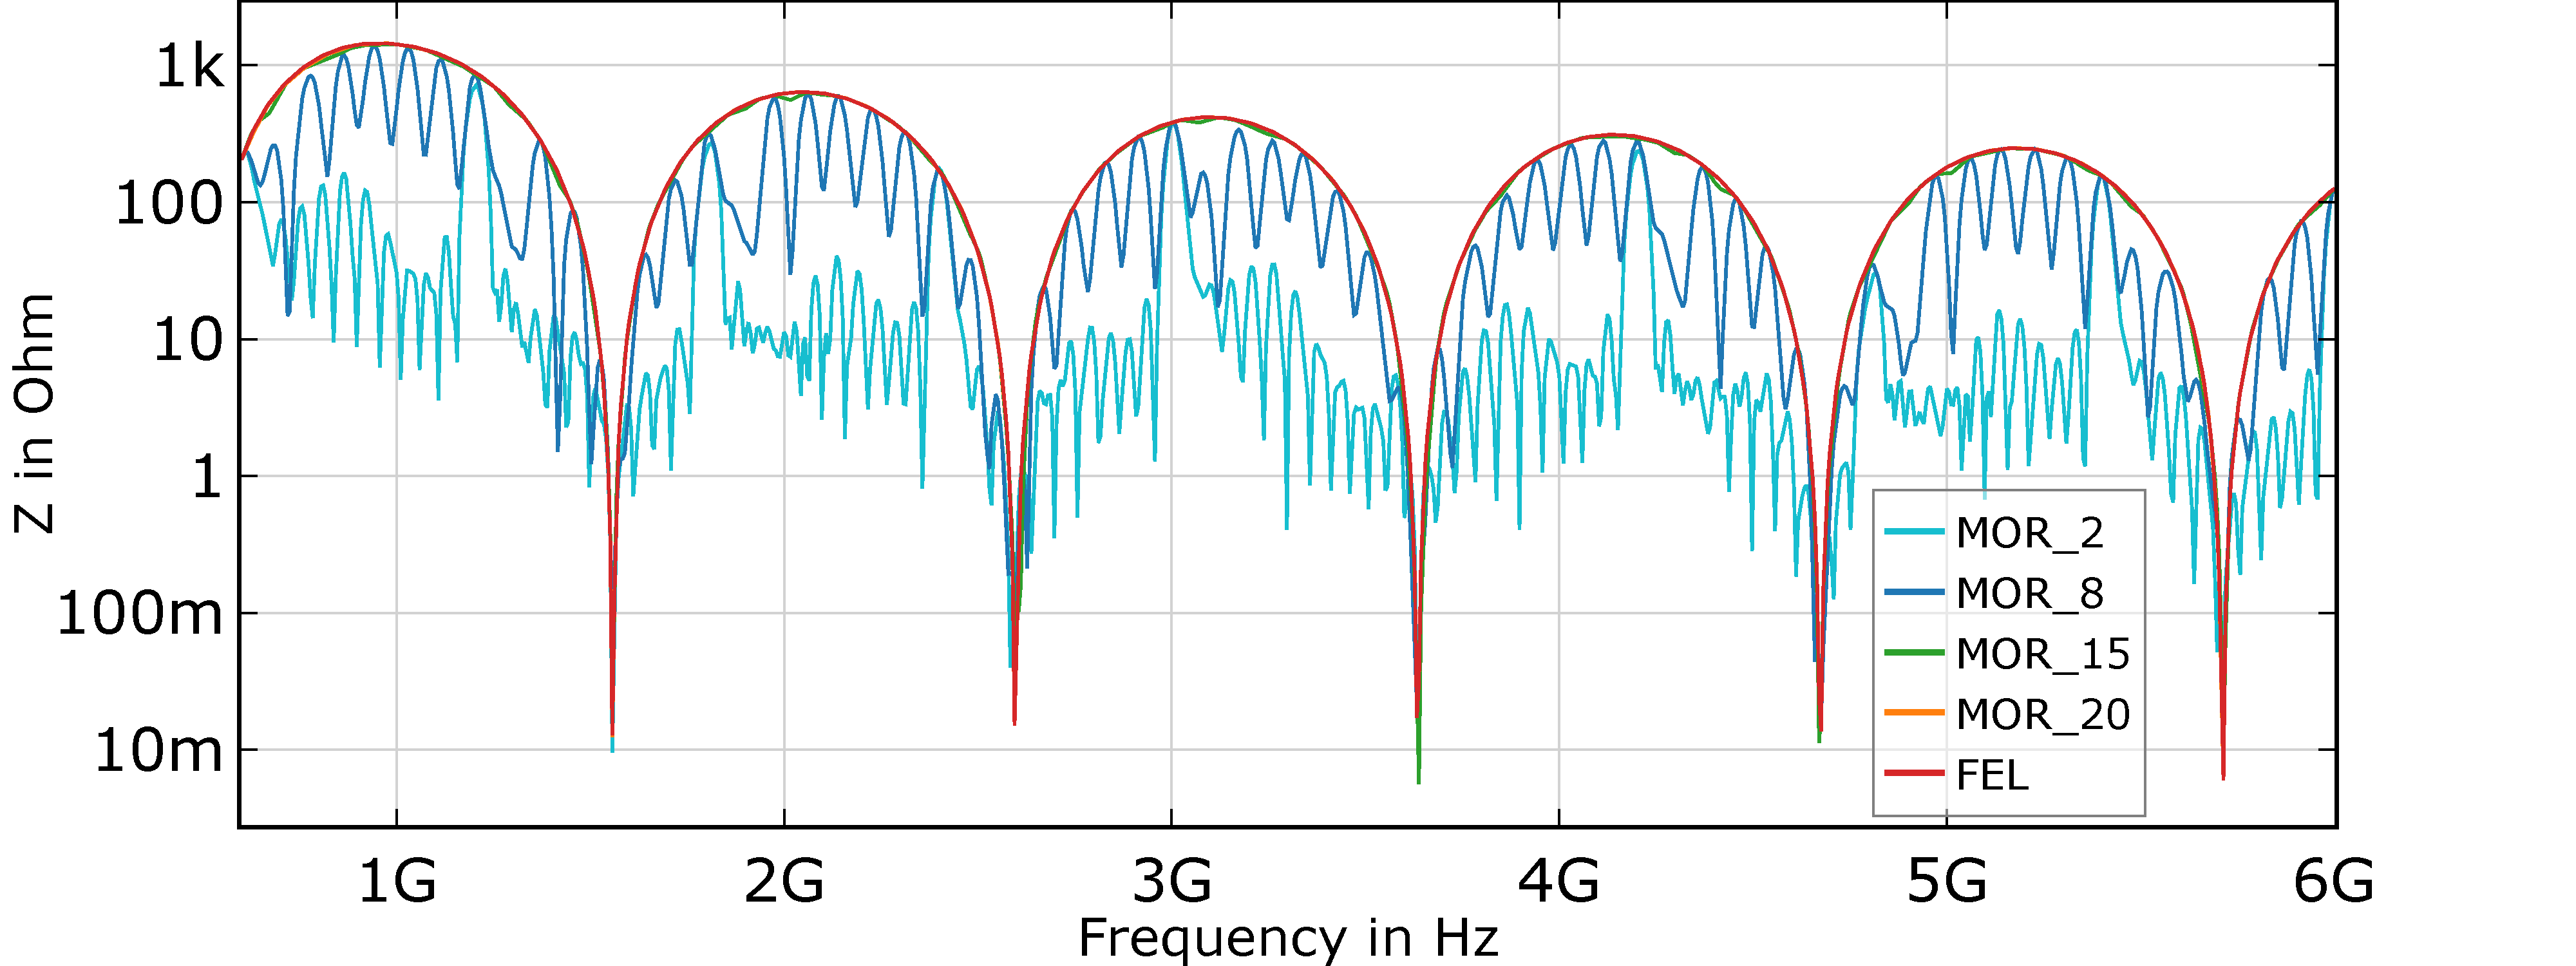
\includegraphics[width=0.5\textwidth]{const_imp_Felis_Py2.pdf}
	\caption{Impedances. }
	\label{}
\end{figure}

\begin{figure}[h]
	\centering
	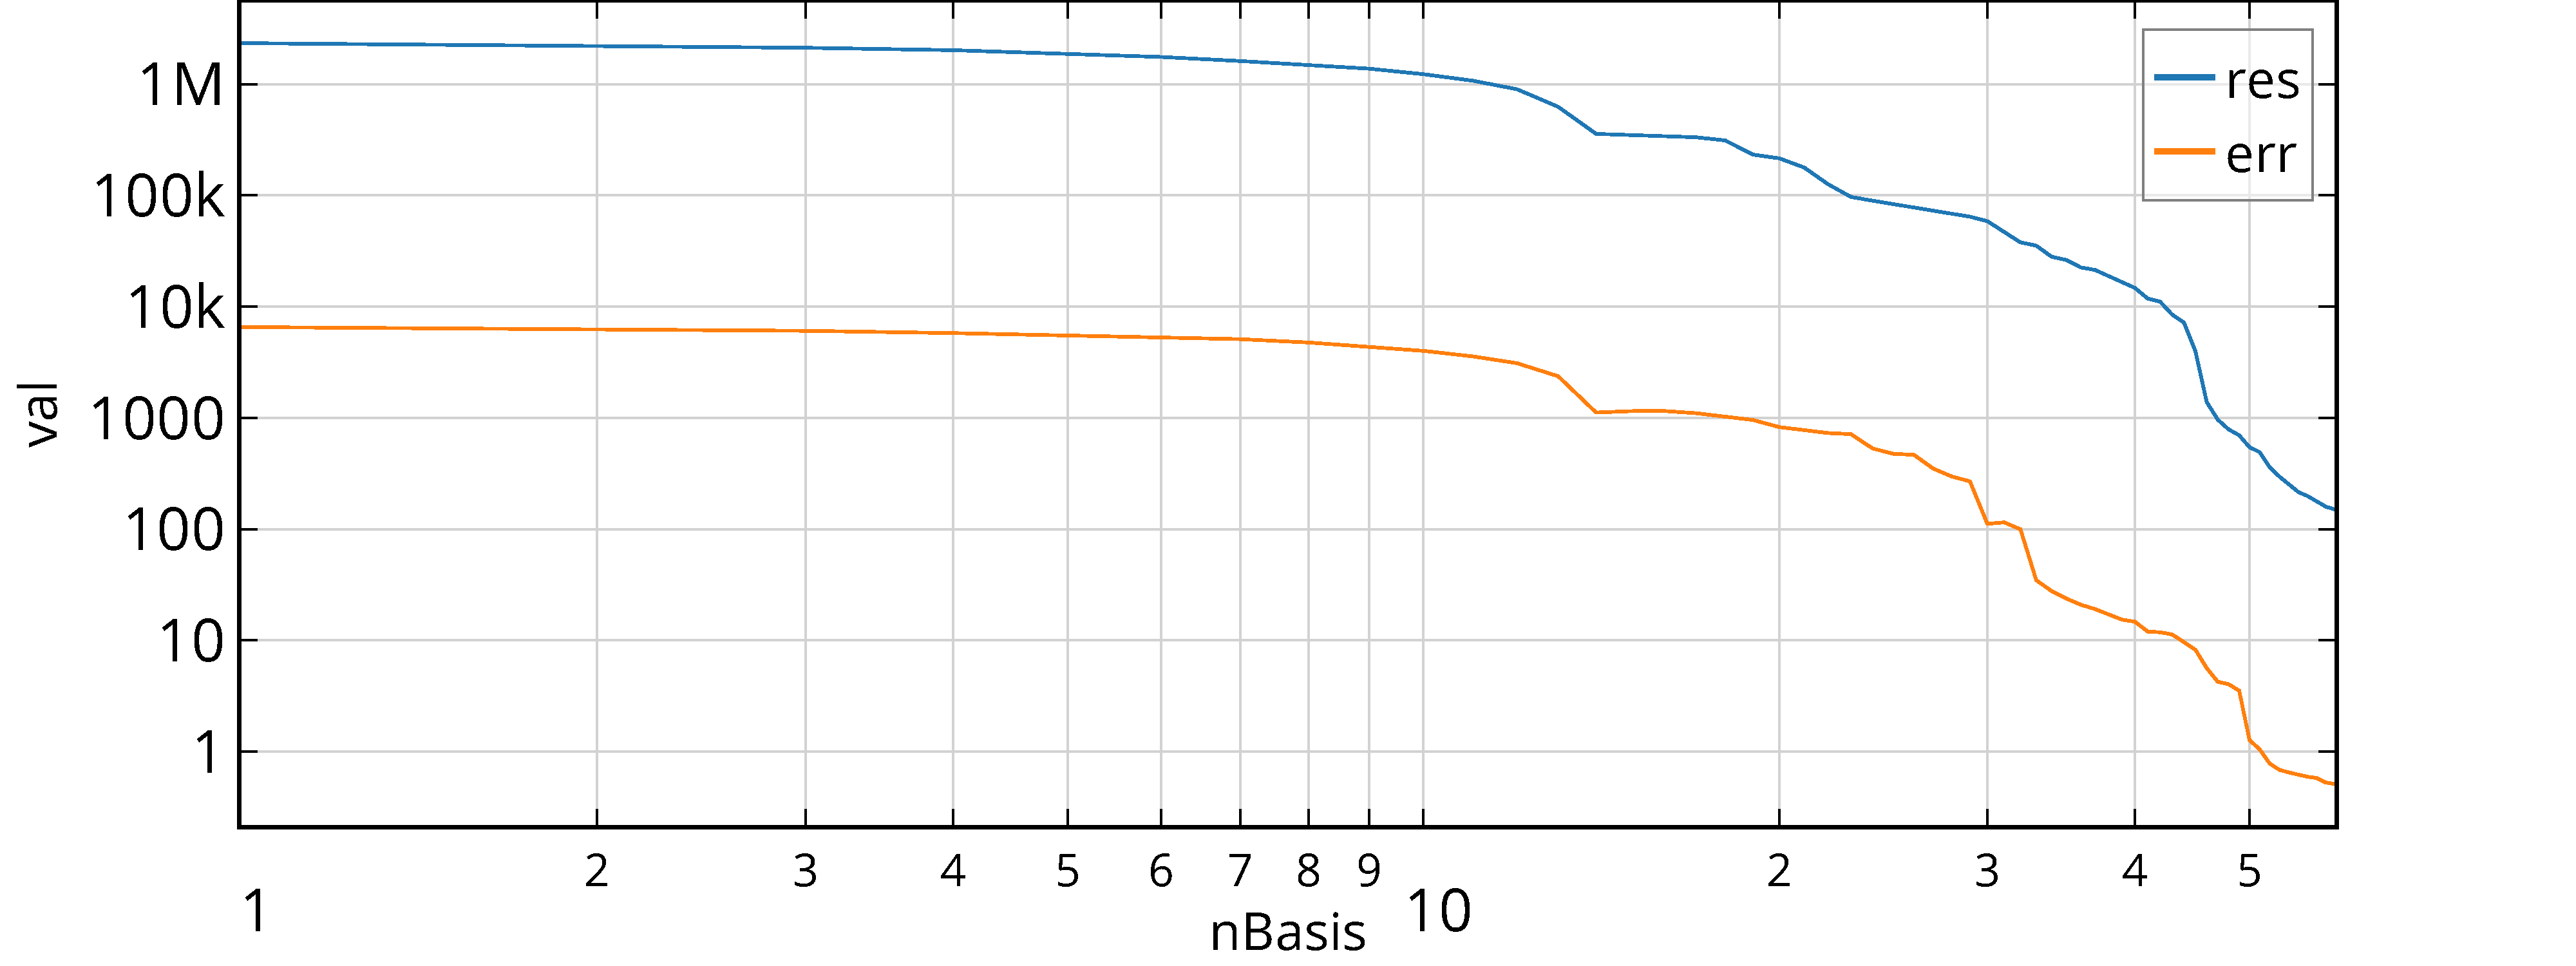
\includegraphics[width=0.5\textwidth]{const_conv_st2_adap_1.pdf}
	\caption{Convergence for the adaptive code. The convergence is a siginificantly faster. The accuracy of the linear case with nB=50 is reached here with nB=30...35.}
	\label{}
\end{figure}

\begin{figure}[h]
	\centering
	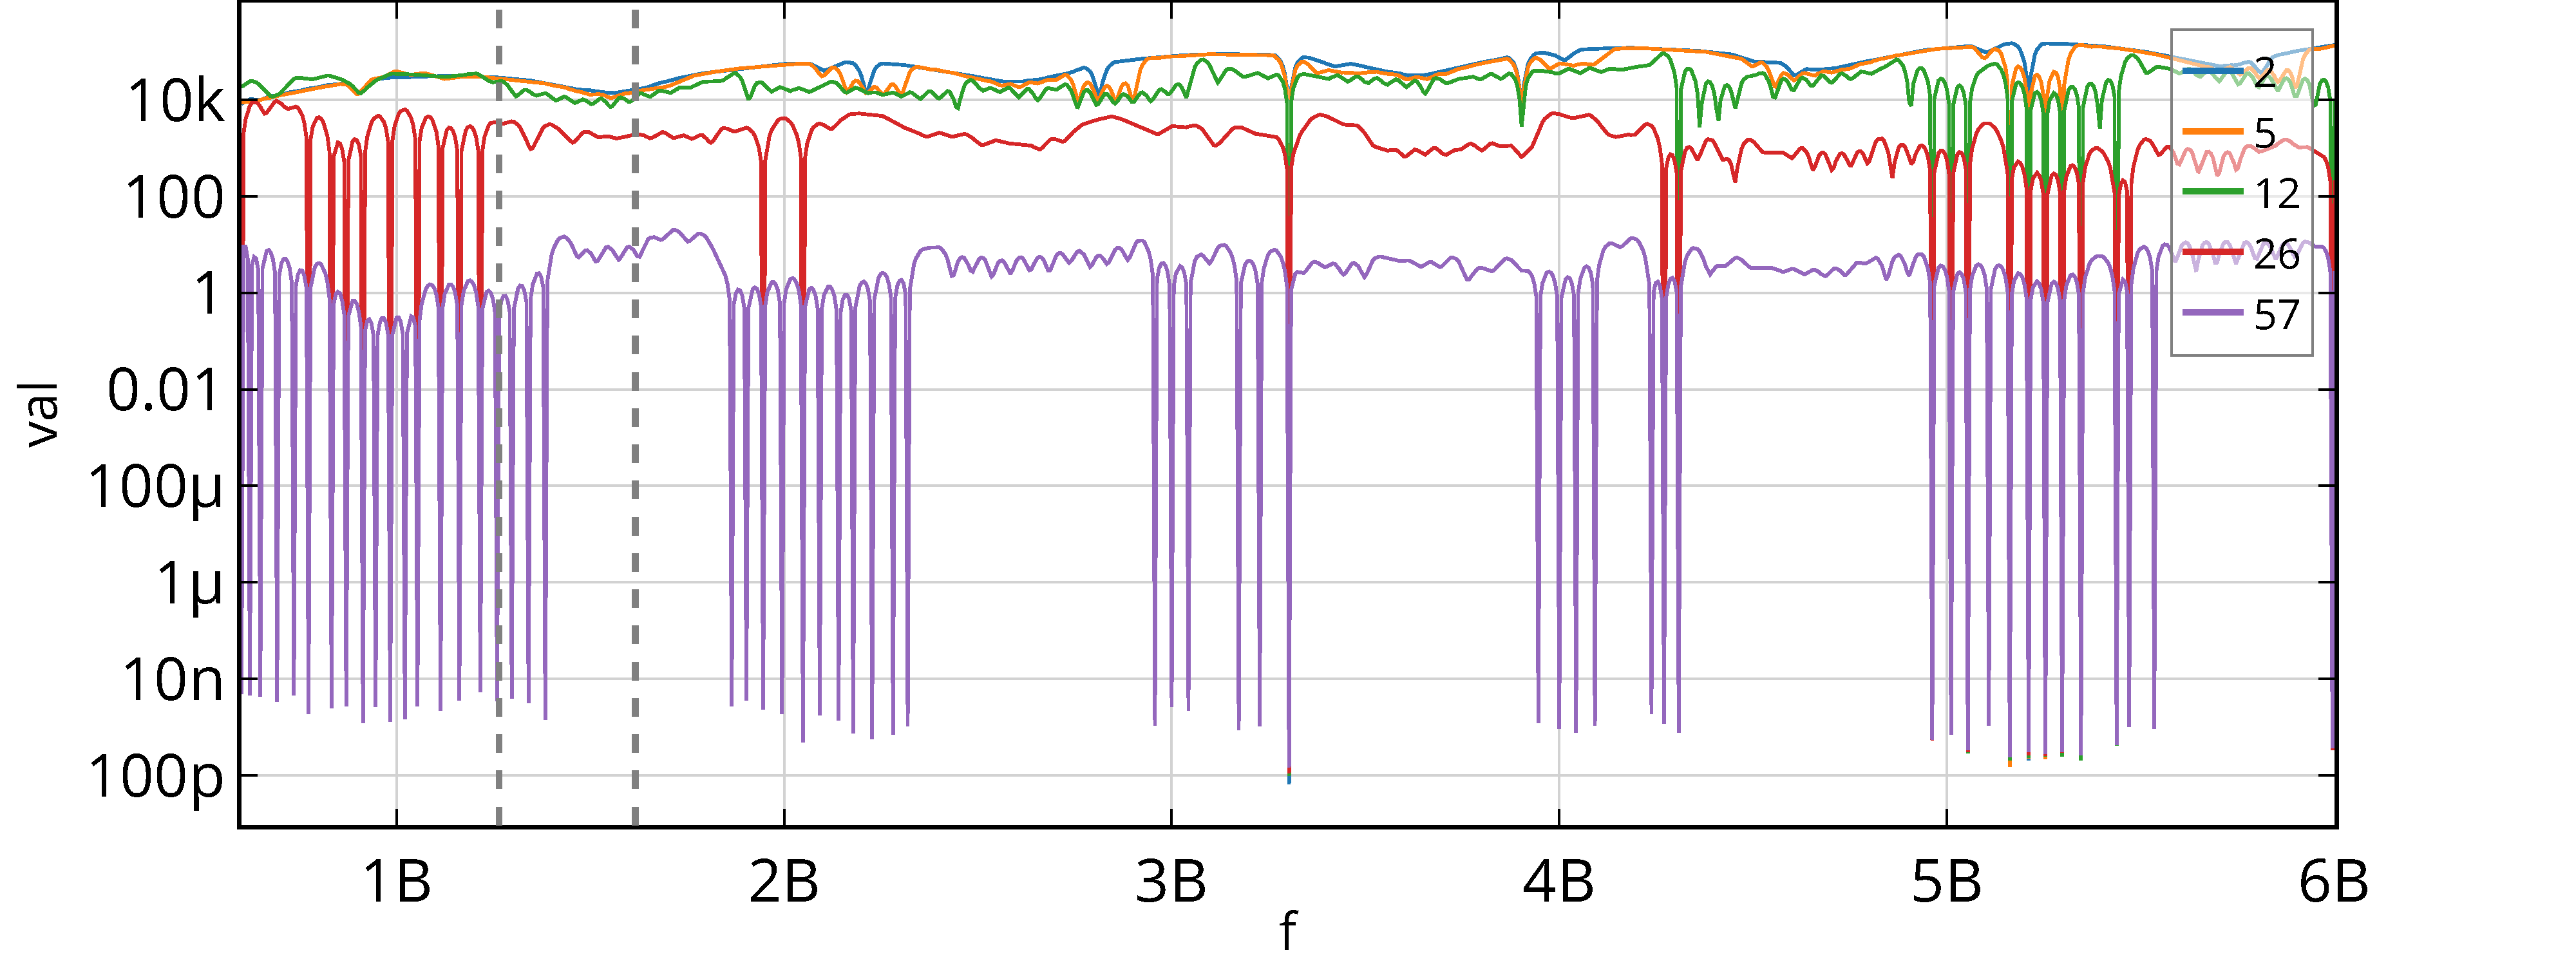
\includegraphics[width=0.5\textwidth]{const_conv_st2_adap_broad1.pdf}
	\caption{convergence over frequency. Even though there are no samples where the impedance is low, there is also a good accuracy.}
	\label{}
\end{figure}


\subsubsection{CubeWire}
Convergence starts at 2nd basis function
Convergence reaches arithmetic accuracy at 11-13 samples with 13 decimals between largest and smallest error/res
fRange=0.2...1GHz

\begin{figure}[h]
	\centering
	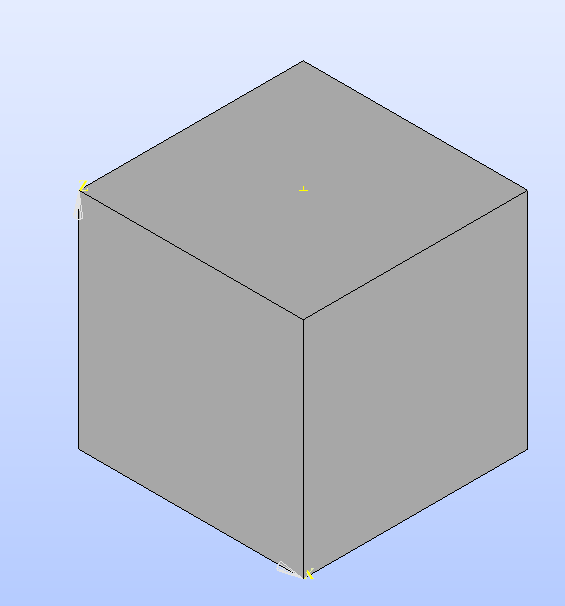
\includegraphics[width=0.5\textwidth]{CubeWireGeo.PNG}
	\caption{Geometry. Surface conductivity=5.8e6 S/m}
	\label{}
\end{figure}














\newpage





\section{time analysis}
This section is based on the commit "Interactive with time measurement".

\begin{figure}[h]
	\centering
	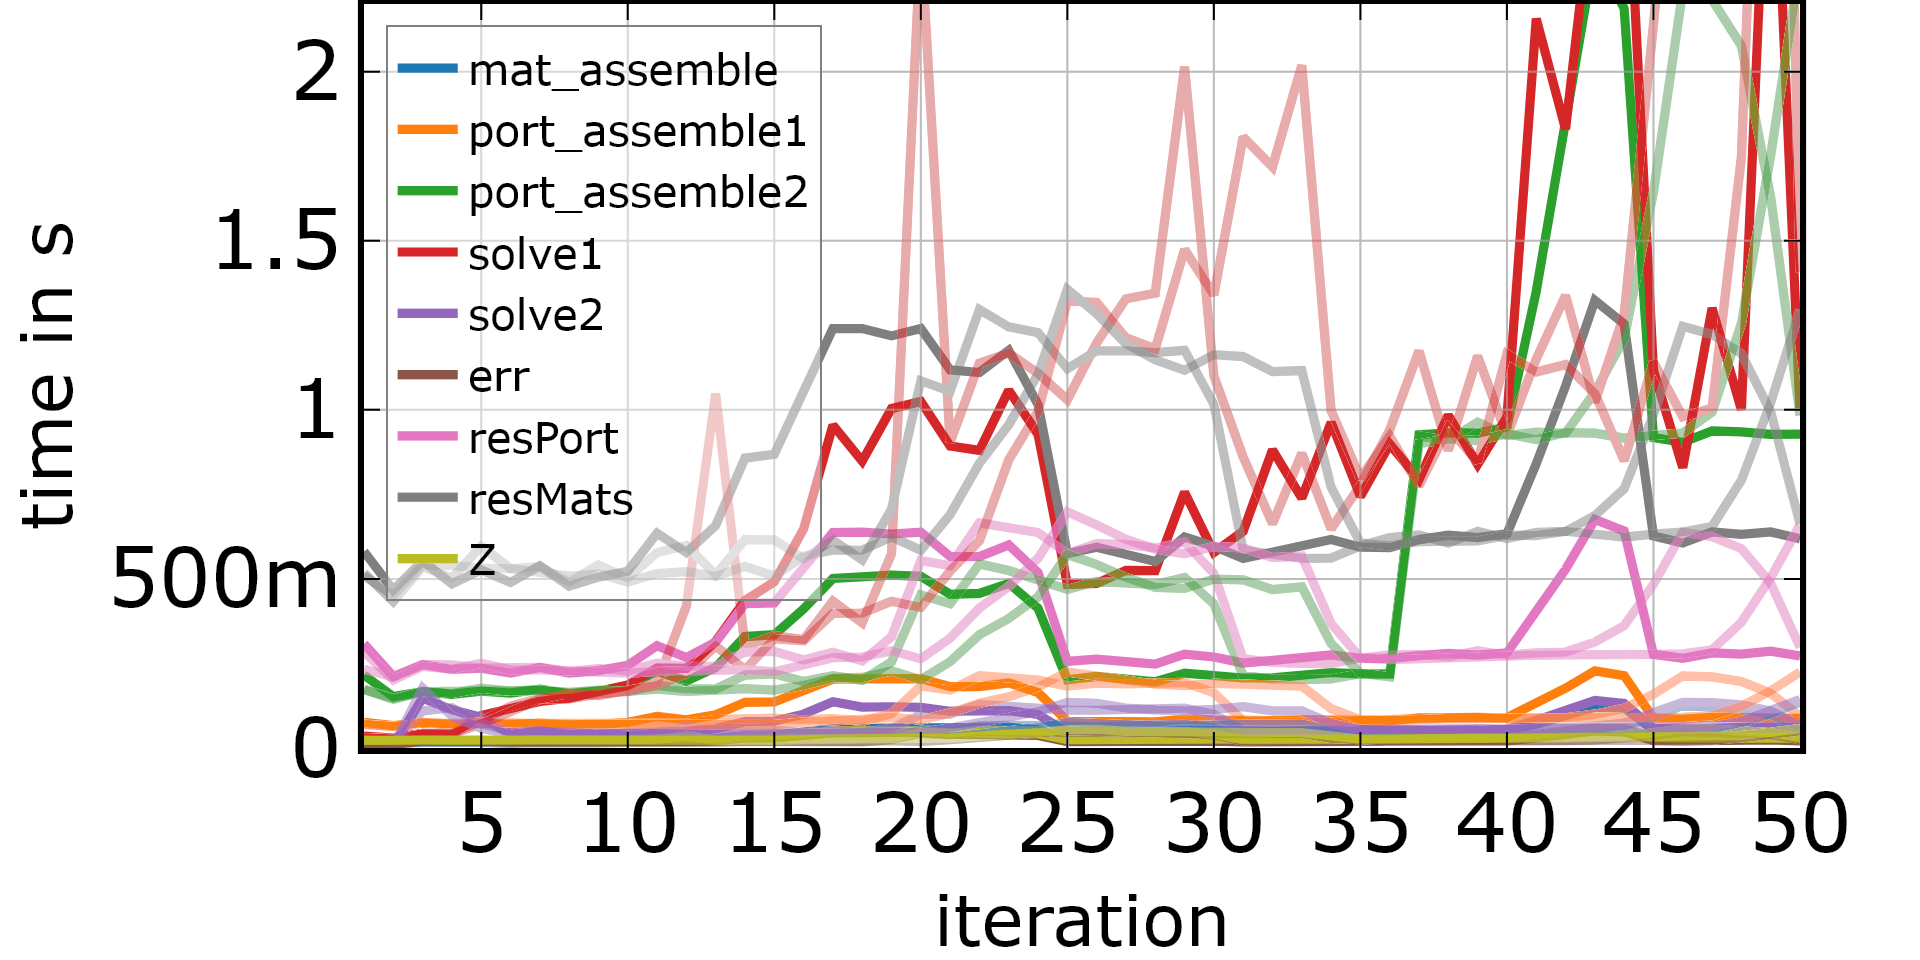
\includegraphics[width=0.5\textwidth]{CubeWire_time_merge1.PNG}
	\caption{Three runtimes for the Cubewire. The opaque lines show one run, the transparent ones two further ones. The increases at around iteration 20 and 40 are likely due to the cooling/turbo boost of the laptop, which can be confirmed by monitoring the task manager. Occasional spikes are distributed randomly, so likely caused by background processes. Important is the sudden increase of port-assemble2 at iteration 37 in all three runs. Also important is solve1, since it is the one which is increasing the quickest.}
	\label{}
\end{figure}


\begin{figure}[h]
	\centering
	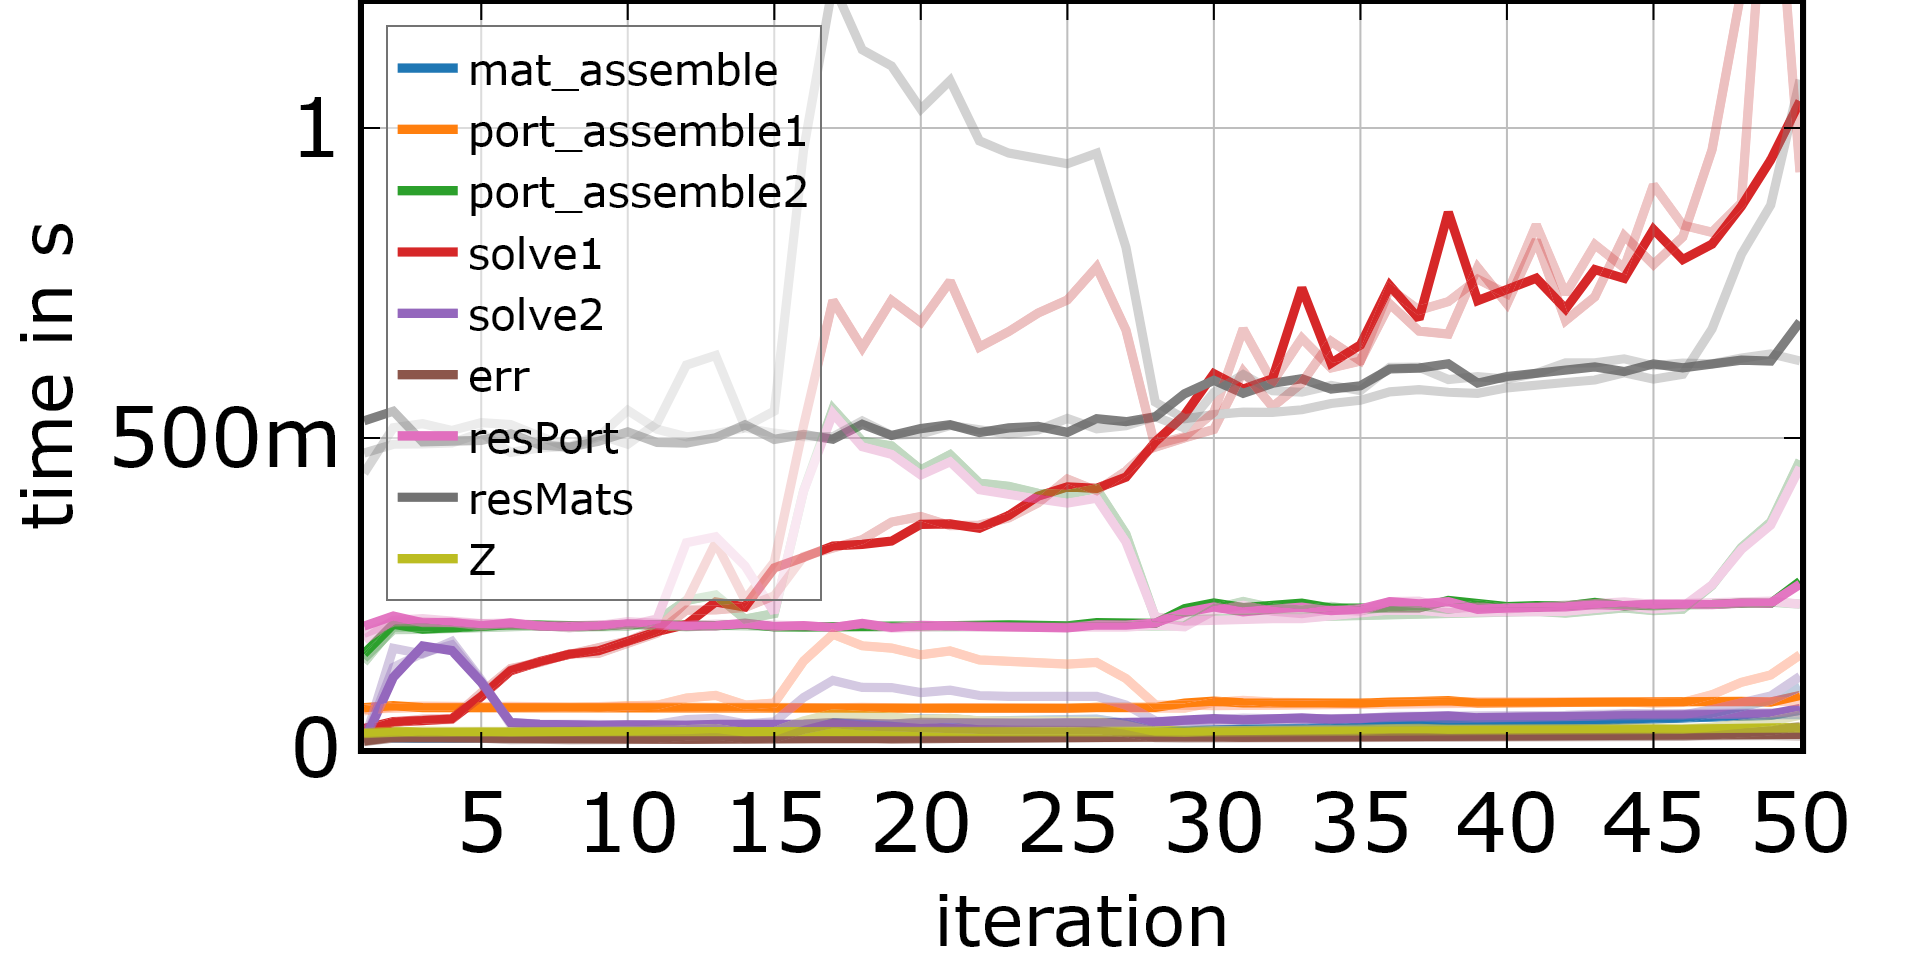
\includegraphics[width=0.5\textwidth]{sqav_time_merge1.PNG}
	\caption{Three runtimes for the square cavity. The opaque lines show one run, the transparent ones two further ones. Similar results as for the cube wire}
	\label{}
\end{figure}



\begin{figure}[h]
	\centering
	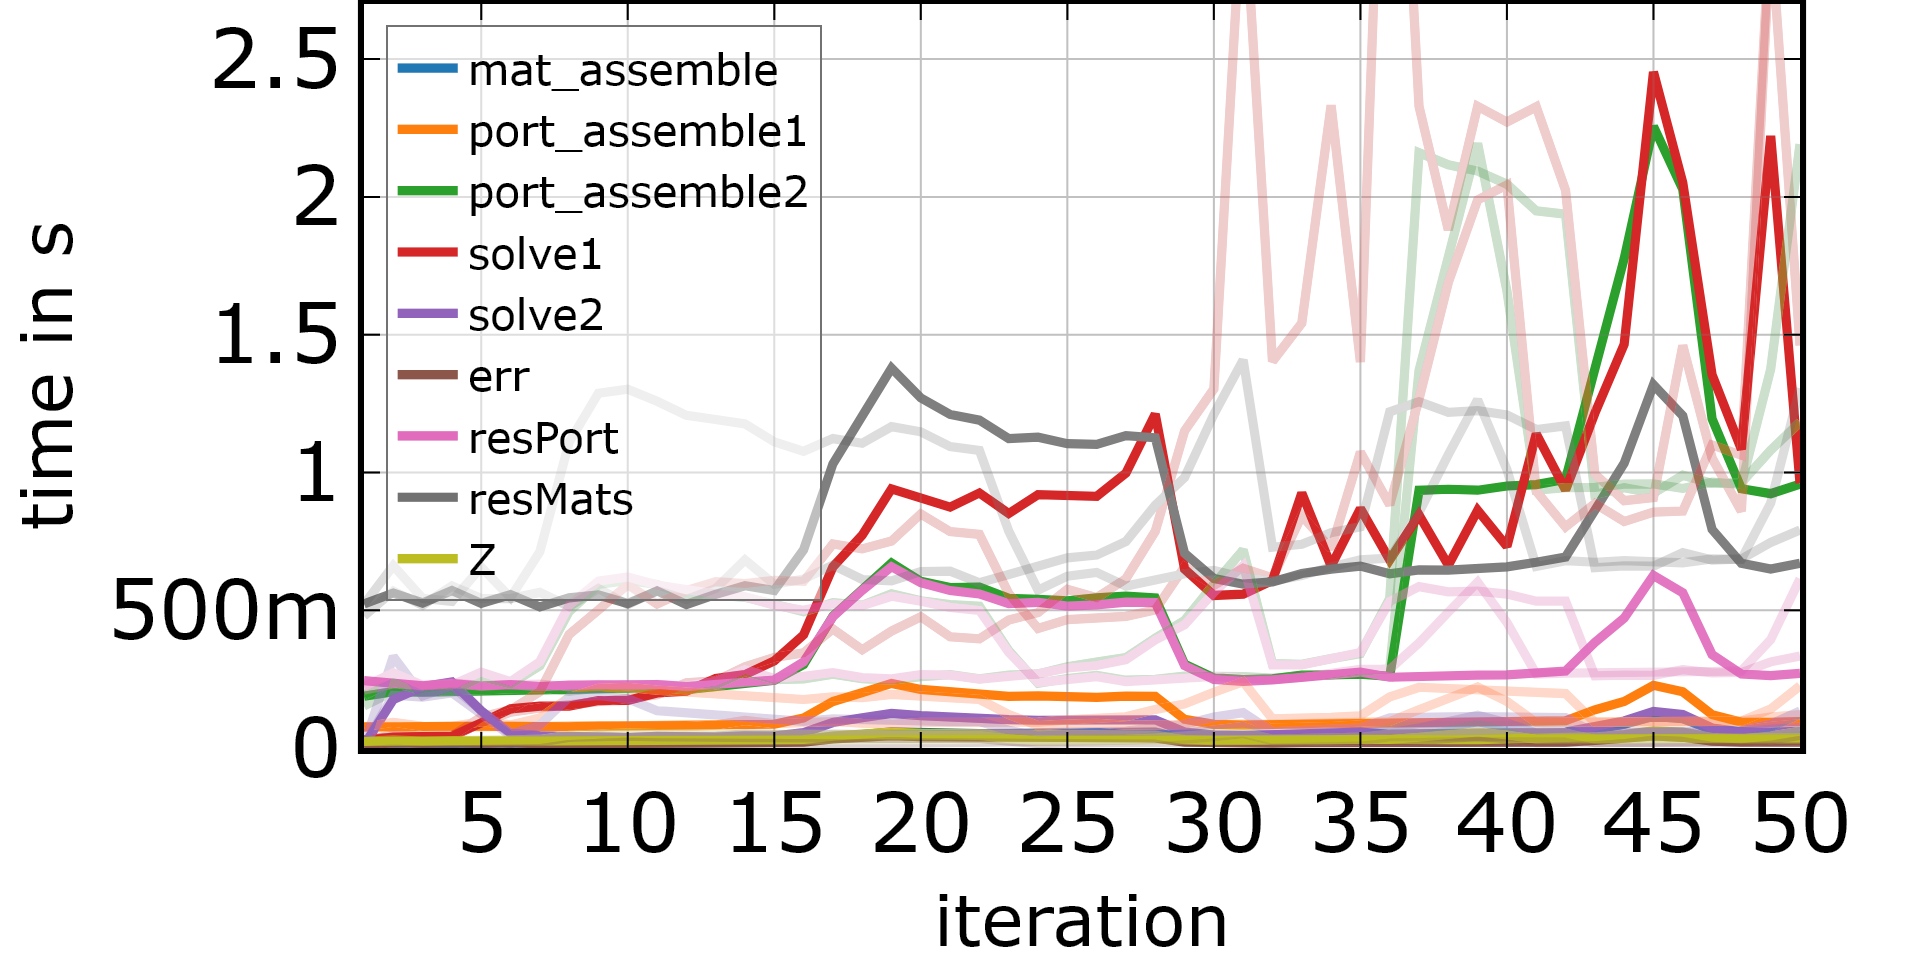
\includegraphics[width=0.5\textwidth]{const_time_merge1.PNG}
	\caption{Three runtimes for the constriction. The opaque lines show one run, the transparent ones two further ones. Similar results as for the cube wire. Here is also a sudden increase of port-assemble2 at iteration 37 in all three runs.}
	\label{}
\end{figure}


\begin{figure}[h]
	\centering
	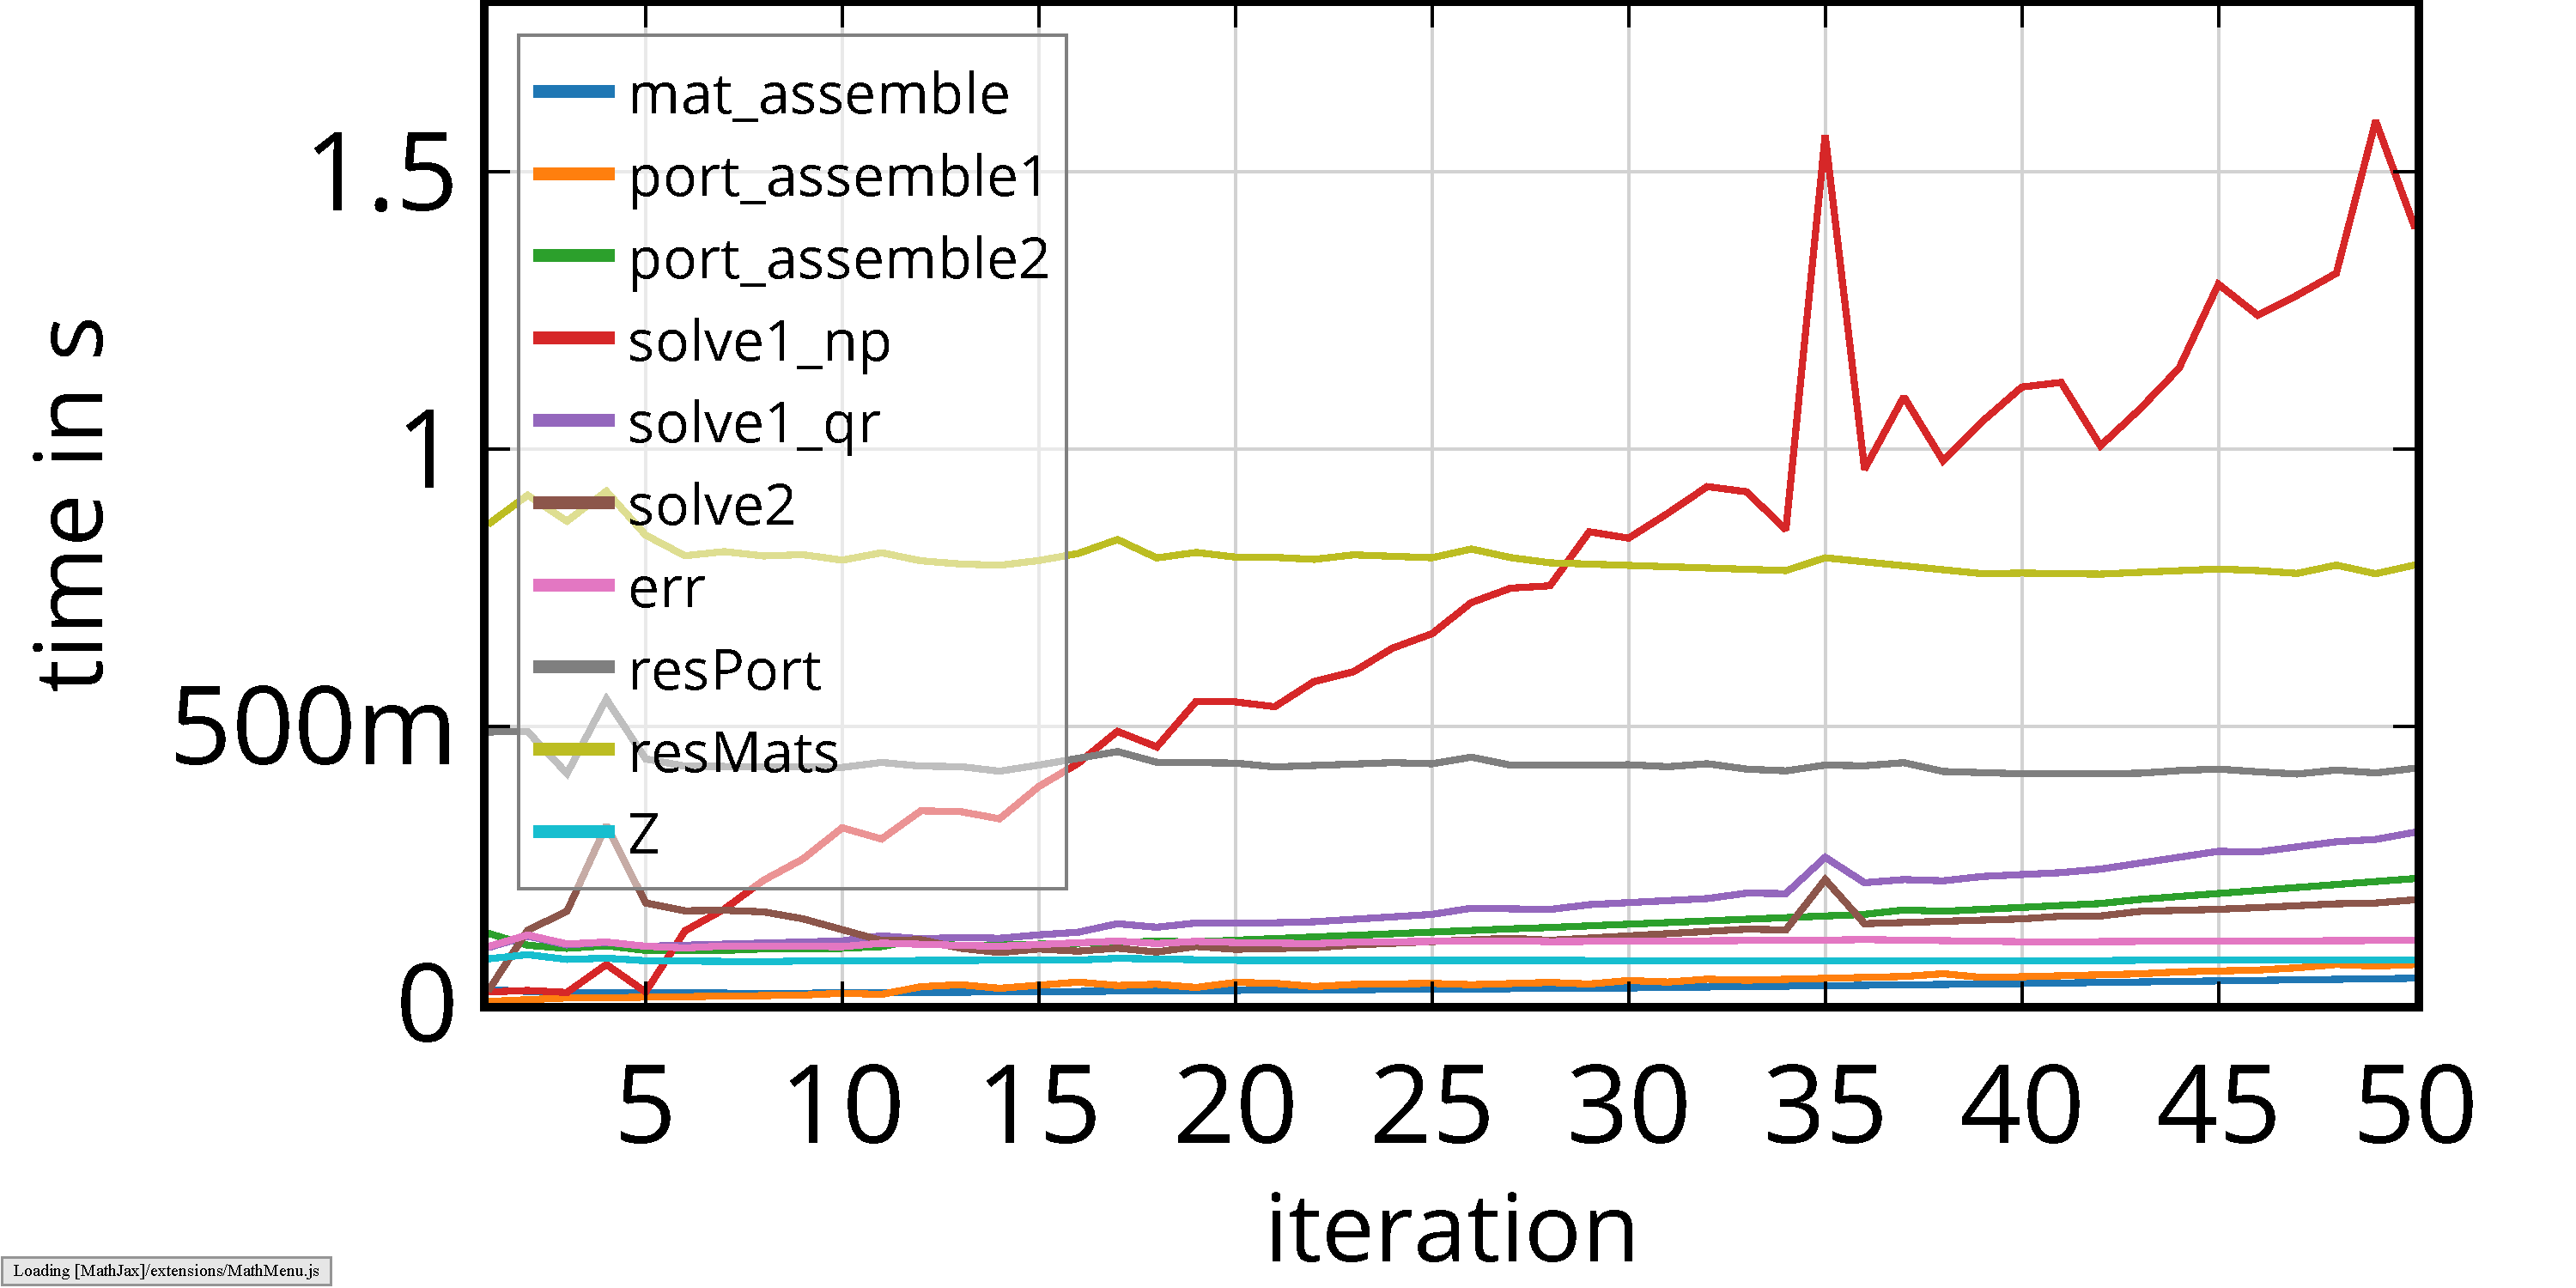
\includegraphics[width=0.5\textwidth]{acc_cav_time_NPvsQR.PNG}
	\caption{Comparison of the numpy linalg solver (red) vs a simple QR decomposition based solver (purple). Clearly the QR solver is more efficient.}
	\label{}
\end{figure}




































% Can use something like this to put references on a page
% by themselves when using endfloat and the captionsoff option.
%\ifCLASSOPTIONcaptionsoff
%  \newpage
%\fi



% trigger a \newpage just before the given reference
% number - used to balance the columns on the last page
% adjust value as needed - may need to be readjusted if
% the document is modified later
%\IEEEtriggeratref{8}
% The "triggered" command can be changed if desired:
%\IEEEtriggercmd{\enlargethispage{-5in}}

% references section

% can use a bibliography generated by BibTeX as a .bbl file
% BibTeX documentation can be easily obtained at:
% http://mirror.ctan.org/biblio/bibtex/contrib/doc/
% The IEEEtran BibTeX style support page is at:
% http://www.michaelshell.org/tex/ieeetran/bibtex/
%\bibliographystyle{IEEEtran}
% argument is your BibTeX string definitions and bibliography database(s)
%\bibliography{IEEEabrv,../bib/paper}
%
% <OR> manually copy in the resultant .bbl file
% set second argument of \begin to the number of references
% (used to reserve space for the reference number labels box)

%\bibliographystyle{IEEEtran}

%\bibliography{literature}



% biography section
% 
% If you have an EPS/PDF photo (graphicx package needed) extra braces are
% needed around the contents of the optional argument to biography to prevent
% the LaTeX parser from getting confused when it sees the complicated
% \includegraphics command within an optional argument. (You could create
% your own custom macro containing the \includegraphics command to make things
% simpler here.)
%\begin{IEEEbiography}[{\includegraphics[width=1in,height=1.25in,clip,keepaspectratio]{mshell}}]{Michael Shell}
% or if you just want to reserve a space for a photo:
%
%\begin{IEEEbiographynophoto}{Frederik Quetscher}
%	Biography text here.
%\end{IEEEbiographynophoto}
%
%
%% if you will not have a photo at all:
%\begin{IEEEbiographynophoto}{Jan Hansen}
%	Biography text here.
%\end{IEEEbiographynophoto}
%
%\begin{IEEEbiography}{Andreas Klaedtke}
%	Biography text here.
%\end{IEEEbiography}
%



% You can push biographies down or up by placing
% a \vfill before or after them. The appropriate
% use of \vfill depends on what kind of text is
% on the last page and whether or not the columns
% are being equalized.

%\vfill

% Can be used to pull up biographies so that the bottom of the last one
% is flush with the other column.
%\enlargethispage{-5in}



% that's all folks
\end{document}


